\chapter{From classical field to quantum field}
\section{Motivation}
\noindent
The state of the field is described by an element $|\psi\rangle$ in Hilbert space. The measurement of the field is described by an operator field $\phi_a(\bm{x})$. The mean value of the measurement of the field is described by Erenfest's theorem
\[\frac{d\langle \psi| \phi_a(\bm{x}) | \psi \rangle}{dt} = -i \langle \psi | [\phi_a(\bm{x}),H_S] | \psi \rangle\]
If $[\phi_a(\bm{x}),H_S]_Q = i[\phi_a(\bm{x}),H_S]_C$, we can reproduce the classical field theory as an average effect of quantum field theory. We also note that the commutation relation here $[A,B] = AB - BA$ obeys the same operation laws as the Poisson bracket in classical field theory. So, what we need here is
\begin{enumerate}
\item the canonical quantization
\[[\phi_a(\bm{x}),\phi_b(\bm{y})] = 0 \quad [\pi^a(\bm{x}),\pi^b(\bm{y})] = 0 \quad [\phi_a(\bm{x}),\pi^b(\bm{y})] = i \delta_a^b \delta(\bm{x}-\bm{y}) \]
\item the same definition of $\mathcal{L}$,$\pi^a$ and $H$ as those in corresponding classical theory.
\end{enumerate}
In Heisenberg picture, we define
\[A_H \equiv U^{-1}(t,t_0) A_S U(t,t_0)\]
Especially,
\[\phi_a(x) \equiv U^{-1}(t,t_0) \phi_a(\bm{x}) U(t,t_0)\]
\[\pi^a(x) \equiv U^{-1}(t,t_0) \pi^a(\bm{x}) U(t,t_0)\]
If $A = f(\phi_a(\bm{x}),\pi^a(\bm{x}),t)$, then we have $A_H = f(\phi_a(x),\pi^a(x),t)$. \\
The canonical quantization can be generalized to the field operator in any time
\[[\phi_a(\bm{x},t),\phi_b(\bm{y},t)] = 0 \quad [\pi^a(\bm{x},t),\pi^b(\bm{y},t)] = 0 \quad [\phi_a(\bm{x},t),\pi^b(\bm{y},t)] = i \delta_a^b \delta(\bm{x}-\bm{y}) \]
The dynamics of the field can be describe by Heisenberg equation
\[\frac{d\phi_a(x)}{dt} = -i[\phi_a(x),H_H]\]
\[\frac{d\pi^a(x)}{dt} = -i[\pi^a(x),H_H]\]
whose form will be equivalent to the classical field equation.

\section{Lorentz invariance in quantum field theory}
\[| \bar{\psi}\rangle = U(\Lambda)| \psi\rangle\]
Scalar fields:
\[\langle \bar{\psi} | \phi(x) | \bar{\psi}\rangle = \langle \psi | \phi(\Lambda^{-1}x) | \psi\rangle\]
\[U^{-1}(\Lambda) \phi(x) U(\Lambda) = \phi(\Lambda^{-1}x)\]
Vector fields:
\[\langle \bar{\psi} | A^{\mu}(x) | \bar{\psi}\rangle = \langle \psi | \Lambda^{\mu}_{\phantom{\mu}\nu} A^{\nu}(\Lambda^{-1}x) | \psi\rangle\]
\[U^{-1}(\Lambda) A^{\mu}(x) U(\Lambda) = \Lambda^{\mu}_{\phantom{\mu}\nu} A^{\nu}(\Lambda^{-1}x)\]
Lorentz invariance means Lagrangian must be a scalar, or more loosely, action must be invariant under Lorentz transformation.

\section{Momentum}
\noindent
The definition of momentum is the same as that in classical theory:
\[T^{\mu \nu} \equiv -\frac{\partial \mathcal{L}}{\partial(\partial_{\mu}\phi_a)} \partial^{\nu} \phi_a + \eta^{\mu \nu} \mathcal{L} \quad \partial_{\mu} T^{\mu \nu} = 0\]
and
\[P^{\mu} \equiv \int T^{0 \mu} d^3 x \quad \frac{d P^{\mu}}{dt} = 0\]
\[P^{0} = H, \quad P^{i} = \int -\pi^a \partial^i \phi_a d^3 x\]
We can get the commutation relation
\begin{eqnarray}
\left[\phi_a,P^{\mu}\right] &=& -i\partial^{\mu} \phi_a \nonumber \\
\left[\pi^a,P^{\mu}\right] &=& -i\partial^{\mu} \pi^a \nonumber \\
\left[P^{\mu},P^{\nu}\right] &=& 0 \nonumber 
\end{eqnarray}
We define the translation operator $T(s)$ by
\[T^{-1}(s) \phi_a(x) T(s) = \phi_a(x-s)\]
then we can derive that
\[T(\epsilon) = 1 - i\epsilon_{\mu} P^{\mu} \quad T(s) = e^{-iP^{\mu}s_{\mu}}\]


\section{Angular Momentum}
\noindent
The definition of angular momentum is the same as that in classical theory:
\[M^{\mu \nu \rho} \equiv x^{\nu}T^{\mu \rho} - x^{\rho} T^{\mu \nu} - \frac{\partial \mathcal{L}}{\partial (\partial_{\mu}\phi_a)}(\Sigma^{\nu \rho})_{a}^{\phantom{a}b}\phi_b\]
and 
\[M^{\nu \rho} \equiv \int M^{0 \nu \rho} d^3 x \quad \frac{dM^{\nu \rho}}{dt} = 0\]
\[M^{\mu \nu} = \int (x^{\mu}T^{0\nu}-x^{\nu}T^{0\mu}-\pi^a(\Sigma^{\mu \nu})_{a}^{\phantom{a}b}\phi_b) d^3 x\]
We also define that
\[M_{L}^{\mu \nu} \equiv \int (x^{\mu}T^{0\nu}-x^{\nu}T^{0\mu}) d^3 x \quad M_S^{\mu \nu} \equiv\int (-\pi^a(\Sigma^{\mu \nu})_{a}^{\phantom{a}b}\phi_b) d^3 x\]
\[(L^{\mu \nu})_a^{\phantom{a}b} \equiv -i(x^{\mu}\partial^{\nu}-x^{\nu}\partial^{\mu})\delta_a^{\phantom{a}b} \quad (S^{\mu \nu})_a^{\phantom{a}b} \equiv -i(\Sigma^{\mu \nu})_a^{\phantom{a}b}\]
We can get the commutation relation
\[M^{\mu \nu} = M_L^{\mu \nu} + M_S^{\mu \nu}\]
\[[\phi_a,M_L^{\mu \nu}] = (L^{\mu \nu})_a^{\phantom{a}b} \phi_b \quad [\phi_a,M_S^{\mu \nu}] = (S^{\mu \nu})_a^{\phantom{a}b} \phi_b\]
\[[\pi^a,M_L^{\mu \nu}] = (L^{\mu \nu})_b^{\phantom{b}a}\pi^{b}  \quad [\pi^a,M_S^{\mu \nu}] = - (S^{\mu \nu})_b^{\phantom{b}a} \pi^b \]
\[[M^{\mu \nu},M^{\rho \sigma}] = i(-\eta^{\nu \rho}M^{\mu \sigma} + \eta^{\sigma \mu}M^{\rho \nu} + \eta^{\mu \rho}M^{\nu \sigma} - \eta^{\sigma \nu}M^{\rho \mu})\] \\
We again define $J_i \equiv \frac{1}{2} \epsilon_{ijk} M^{jk}$ and $K_i \equiv M^{i0}$, the communication relation can be written as
\begin{eqnarray}
\left[J_i,J_j\right] &=& i\epsilon_{ijk}J_k \nonumber \\
\left[J_i,K_j\right] &=& i\epsilon_{ijk}K_k \nonumber \\
\left[K_i,K_j\right] &=& -i\epsilon_{ijk}J_k \nonumber
\end{eqnarray} \\
Further more,
\[[P^{\mu},M^{\rho \sigma}] = i(\eta^{\mu \sigma}P^{\mu} - \eta^{\mu \rho}P^{\sigma})\]
\begin{eqnarray}
\left[J_i,H\right] &=& 0 \nonumber \\
\left[J_i,P_j\right] &=& i\epsilon_{ijk}P_k \nonumber \\
\left[K_i,H\right] &=& iP_i \nonumber \\
\left[K_i,P_j\right] &=& i\delta_{ij}H \nonumber
\end{eqnarray}
At last, we also define $L_i \equiv \frac{1}{2} \epsilon_{ijk} M_L^{jk}$ and $S_i \equiv \frac{1}{2} \epsilon_{ijk} M_S^{jk}$. So
\begin{eqnarray}
\left[L_i,S_j\right] &=& 0 \nonumber \\
\left[S_i,P_j\right] &=& 0 \nonumber \\
\left[L_i,P_j\right] &=& i\epsilon_{ijk}P_k \nonumber
\end{eqnarray}
We define the rotation operator $U(\Lambda)$ by
\[U^{-1}(\Lambda) \phi_a(x) U(\Lambda) = \mathcal{S}_{a}^{\phantom{a}b}\phi_b(\Lambda^{-1}x)\]
where
\[\mathcal{S}_{a}^{\phantom{a}b} = \delta_{a}^{\phantom{a}b}+\frac{i}{2} \delta \omega_{\alpha \beta} (S^{\alpha \beta})_{a}^{\phantom{a}b} \]
We can derive that
\[U(1+\delta \omega) = 1 + \frac{i}{2} \delta \omega_{\mu \nu} M^{\mu \nu} \quad U(\Lambda) = e^{\frac{i}{2} \theta_{\mu \nu} M^{\mu \nu}}\]
\[U^{-1}(\Lambda) P^{\mu} U(\Lambda) = \Lambda^{\mu}_{\phantom{\mu}\nu} P^{\nu}\]
\[U^{-1}(\Lambda) M^{\mu \nu} U(\Lambda) = \Lambda^{\mu}_{\phantom{\mu}\rho} \Lambda^{\nu}_{\phantom{\nu}\sigma}M^{\rho \sigma}\]

\section{Anticommutation relation}
\noindent
We define the anticommutation relation of operators as $\{A,B\} \equiv AB + BA$. Suppose that the field operator and its canonical momentum operator has the following anticommutation relation
\[\{\phi_a(\bm{x},t),\phi_b(\bm{y},t)\} = 0 \quad \{\pi^a(\bm{x},t),\pi^b(\bm{y},t)\} = 0 \quad \{\phi_a(\bm{x},t),\pi^b(\bm{y},t)\} = i \delta_a^b \delta(\bm{x}-\bm{y}) \]
If the operator $A$ composes of the terms like $\pi^a \mathcal{E}_a^{\phantom{a}b} \phi_b$, we can show that the value of $[\phi_a,A]$ and $[\pi^a,A]$ is the same as those in the theory quantized with commutation relation. It is easy to verify that the operator $P^i$ and $M_S^{\mu \nu}$ has the required form. The form of $H$ is determined by the specific theory. As we can see later, the Hamiltonian of Dirac field  has the required form. When it is quantized with anticommutation relation, the commutation relation between field operator and momentum, angular momentum discussed in previous section will be hold automatically. 

\chapter{Spin 0 Field}
\section{Klein-Gordon field}
\subsubsection{Lagrangian}
\[\mathcal{L} = -\frac{1}{2} \partial^{\mu} \phi \partial_{\mu} \phi -\frac{1}{2}m^2 \phi^2 + \Omega_0\]
\subsubsection{Field equation}
\[(\partial^{\mu} \partial_{\mu} - m^2) \phi = 0\]
\subsubsection{Hamiltonian}
\[\pi = \dot{\phi}\]
\[\mathcal{H} = \frac{1}{2} \pi^2 + \frac{1}{2} (\nabla \phi)^2 + \frac{1}{2} m^2 \phi^2-\Omega_0\]
\[H = \int \mathcal{H} d^3 x\]
\subsubsection{Momentum and angular momentum}
\[T^{\mu \nu} = \partial^{\mu} \phi \partial^{\nu} \phi - \eta^{\mu \nu}(\frac{1}{2}\partial^{\mu}\phi \partial_{\mu} \phi + \frac{1}{2}m^2 \phi^2 -\Omega_0)\]
\[P^0 = H \quad P^i = \int -\pi \nabla^i \phi d^3 x\]
\[J_k = \int - \pi \epsilon_{ijk} x^{j} \nabla^{k} \phi d^3 x\]

\section{Canonical quantization Formulation}
\subsubsection{Canonical quantization}
\begin{eqnarray}
\left[\phi(\bm{x},t),\phi(\bm{y},t)\right] &=& 0 \nonumber \\
\left[\pi(\bm{x},t),\pi(\bm{y},t)\right] &=& 0 \nonumber \\
\left[\phi(\bm{x},t),\pi(\bm{y},t)\right] &=& i \delta(\bm{x}-\bm{y}) \nonumber
\end{eqnarray}
\subsubsection{Fourier expansion}
\[\phi(\bm{x},t) = \int \widetilde{dk} \left[ a(\bm{k})e^{ikx} + a^{\dagger}(\bm{k})e^{-ikx} \right]\]
\[\pi(\bm{x},t) = -i \int  \widetilde{dk} \omega \left[ a(\bm{k})e^{ikx} - a^{\dagger}(\bm{k})e^{-ikx} \right]\]
Here, $k^2 = \bm{k}^2 - \omega^2 = -m^2$, $kx = \bm{k}\cdot \bm{x} - \omega t$, $\widetilde{dk} = \frac{d^3k}{(2\pi)^3 2\omega}$
\[a(\bm{k}) = \int d^3 x e^{-ikx}(i\pi+\omega \phi)\]
\[a^{\dagger}(\bm{k}) = \int d^3 x e^{ikx}(-i\pi+\omega \phi)\]
\begin{eqnarray}
\left[a(\bm{p}),a(\bm{q})\right] &=& 0 \nonumber \\
\left[a^{\dagger}(\bm{p}),a^{\dagger}(\bm{q})\right] &=& 0 \nonumber \\
\left[a(\bm{p}),a^{\dagger}(\bm{q})\right] &=& (2\pi)^3 2\omega \delta(\bm{p}-\bm{q}) \nonumber
\end{eqnarray}
\subsubsection{Operator represented by $a$ and $a^{\dagger}$}
\[H=\int \widetilde{dk}\, \omega\, a^{\dagger}(\bm{k})a(\bm{k}) + (\mathcal{E}_0 - \Omega_0)V \quad \mathcal{E}_0 = \frac{1}{2}(2\pi)^{-3}\int d^3 k \,\omega\]
\[P^{i}=\int \widetilde{dk}\, k^{i}\, a^{\dagger}(\bm{k})a(\bm{k}) \]
\subsubsection{Particles}
\[[H,a(\bm{k})] = -\omega a(\bm{k}) \quad [H,a^{\dagger}(\bm{k})] = \omega a^{\dagger}(\bm{k})\]
\[[P^i,a(\bm{k})] = -k^i a(\bm{k}) \quad [P^i,a^{\dagger}(\bm{k})] = k^i a^{\dagger}(\bm{k})\]
Let $|p\rangle = a^{\dagger}(\bm{p})|0\rangle $,so
\[H |p\rangle = \omega_p|p\rangle \quad P^i |p\rangle = p^i|p\rangle\]
So, we interpret the state $|\bm{p}\rangle$ as the momentum eigenstate of a single particle of mass $m$. We can also show that 
$J_i|\bm{p} = 0\rangle = 0$, so the particle carries no internal angular momentum.
\subsubsection{Causality}
\noindent
The amplitude for a particle to propagate from $y$ to $x$ is $\langle 0 | \phi(x) \phi(y) | 0 \rangle$, denoted by $D(x-y)$.
\[D(x-y) = \int \widetilde{dk} e^{ik(x-y)}\]
\[[\phi(x),\phi(y)] = D(x-y) -D(y-x)\]
If $x-y$ is space-like, a continuous Lorentz transformation can take $(x-y)$ to $-(x-y)$. So $[\phi(x),\phi(y)] =0$ for space-like $x-y$. A measurement performed at one point can not affect a measurement at another point whose separation is space-like.
\subsubsection{The Klein-Gordon propagator}
\[D_R(x-y) \equiv \theta(x^0-y^0) \langle 0 | [\phi(x) \phi(y)] | 0 \rangle = \int \frac{d^4 p}{(2\pi)^4} \frac{-i}{p^2+m^2} e^{ip(x-y)}\]
\begin{figure}[!h]
\centering
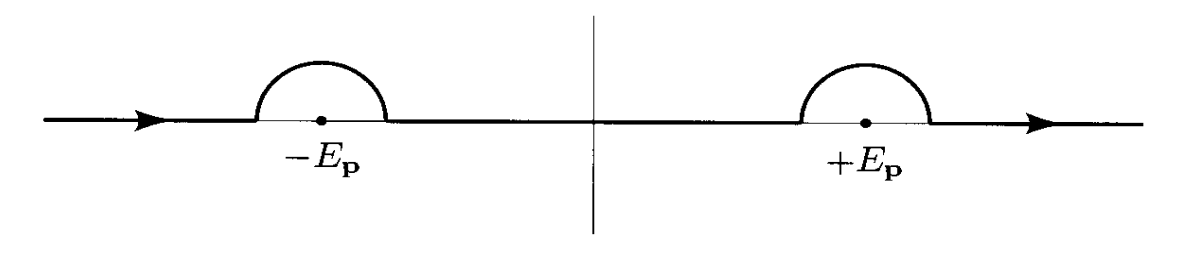
\includegraphics[height=2.55cm ,width=11.88cm]{QFT1/Green1.png}
\caption{Retarded Green Function}
\end{figure}
\[(\partial^2-m^2) D_R(x-y) = i \delta(x-y)\]
\[D_F(x-y) \equiv \langle 0 | T\phi(x) \phi(y) | 0 \rangle = \int \frac{d^4 p}{(2\pi)^4} \frac{-i}{p^2+m^2-i\epsilon} e^{ip(x-y)}\]
Here, $T$ stands for time ordering, placing all operators evaluated at later times to the left.
\begin{figure}[!h]
\centering
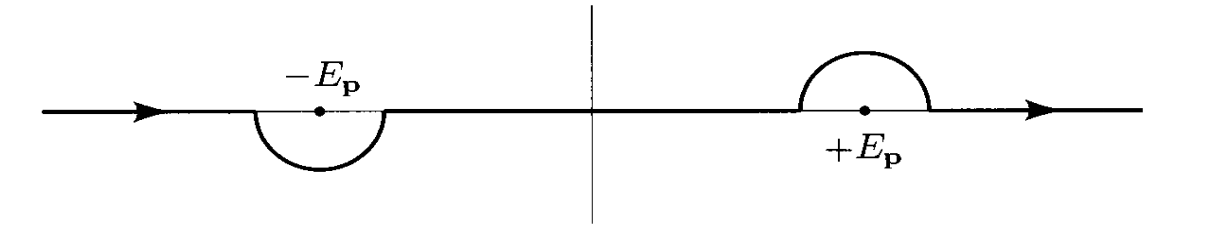
\includegraphics[height=2.38cm ,width=12.24cm]{QFT1/Green2.png}
\caption{Feynman Green Function}
\end{figure}

\section{Perturbation theory for canonical quantization}
\[\mathcal{L} = -\frac{1}{2}\partial_{\mu} \phi \partial^{\mu} \phi -\frac{1}{2}m_0^2 \phi^2 -\frac{\lambda_0}{4!}\phi^4\]
\[H = H_0 + H_{int} \quad H_{int} = \int d^3 x \frac{\lambda_0^4}{4!} \phi^4 (\bm{x})\]
\subsection{Perturbation expansion of correlation functions}
\begin{note}
The ground state of the interaction field theory is denoted by $| \Omega \rangle$, the ground state of the free field theory is denoted by $| 0 \rangle$. The zero of energy is defined by $H_0 | 0 \rangle =0$ and $E_0 = \langle \Omega | H | \Omega \rangle$.
\end{note}
\[\phi(t_0,\bm{x}) = \int \frac{d^3p}{(2\pi)^3}( a(\bm{p})e^{i\bm{p}\cdot\bm{x}} + a^{\dagger}(\bm{p})e^{-i\bm{p}\cdot\bm{x}})\]
\[\phi(t,\bm{x}) = e^{iH(t-t_0)} \phi(t_0,\bm{x}) e^{-iH(t-t_0)}\]
\[\phi_I(t,\bm{x}) \equiv e^{iH_0(t-t_0)} \phi(t_0,\bm{x}) e^{-iH_0(t-t_0)}\]
\[H_I(x) = \int d^3x \frac{\lambda_0^4}{4!} \phi_I^4\]
The perturbation expansion of correlation functions is
\[\langle \Omega | T \{ \phi(x) \phi(y) \} | \Omega \rangle = \lim_{T \to \infty(1-i\epsilon)} \frac{\langle 0 | T \left\{ \phi_I(x) \phi_I(y) \mathrm{exp} \left[ -i \int_{-T}^{T} dt H_I \right]\right\} | 0 \rangle}{\langle 0 | T \left\{ \mathrm{exp} \left[ -i \int_{-T}^{T} dt H_I \right]\right\} | 0 \rangle}\]
The proof can be found in chapter 4.2 of \emph{An introduction to quantum field theory (M.E.Peskin \& D.V.Schroeder)}
\\

\begin{newthem}[Wick's theorem]
\[T \left\{ \phi(x_1) \phi(x_2) \cdots \phi(x_n)\right\} = N \left\{ \phi(x_1) \phi(x_2) \cdots \phi(x_n) + \mbox{ all possible contractions }\right\} \]
Normal order : all the $a$'s are to the right of all the $a^{\dagger}$.
\end{newthem}
\noindent
The proof can be found in chapter 4.3 of \emph{An introduction to quantum field theory (M.E.Peskin \& D.V.Schroeder)}
\begin{example}
\begin{eqnarray}
\langle 0 | T \left\{ \phi_I(x_1) \phi_I(x_2) \phi_I(x_3) \phi_I(x_4)\right\}| 0 \rangle &=& D_F(x_1-x_2)D_F(x_3-x_4) \nonumber \\
&+& D_F(x_1-x_3)D_F(x_2-x_4) \nonumber \\
&+& D_F(x_1-x_4)D_F(x_2-x_3) \nonumber
\end{eqnarray}
\end{example}

\subsection{Feynman diagram}
Expand $\langle 0 | T \left\{ \phi_I(x) \phi_I(y) \mathrm{exp} \left[ -i \int_{-T}^{T} dt H_I \right]\right\} | 0 \rangle$ to the first order of $\lambda_0$
\begin{eqnarray}
& &\langle 0 | T \left\{ \phi_I(x) \phi_I(y) \frac{-i\lambda_0}{4!} \int dz^4 \phi_I(z) \phi_I(z) \phi_I(z) \phi_I(z) \right\} | 0 \rangle \nonumber \\
&=& 3 \cdot (\frac{-i\lambda_0}{4!}) D_F(x-y) \int d^4 z D_F(z-z) D_F(z-z) \nonumber \\
&+& 12 \cdot (\frac{-i\lambda_0}{4!}) \int d^4 z  D_F(x-z) D_F(y-z) D_F(z-z) \nonumber
\end{eqnarray}
It can be represented by the so called Feynman diagram.
\begin{figure}[!h]
\centering
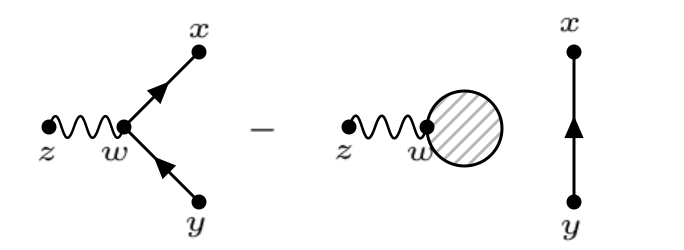
\includegraphics[height=1.98cm ,width=10.68cm]{QFT1/FD1.png}
\caption{Feynman diagram representation of perturbation expansion}
\end{figure}
\\
The symmetry factor of the first diagram is $S = \frac{4!}{3} = 8$.
The symmetry factor of the second diagram is $S = \frac{4!}{12} = 2$.
The Feynman rules for $\phi^4$ theory are:
\begin{enumerate}
\item For each propagator, $P = D_F(x-y)$
\item For each vertex, $V = (-i\lambda_0)\int d^4z$
\item For each external point, $E=1$
\item Divided by the symmetry factor
\end{enumerate}
At last, we can prove that
\[\langle \Omega | T \{ \phi_I(x_1) \phi_I(x_2) \cdots \phi_I(x_n) \} | \Omega \rangle = \mbox{ sum of all E-connected diagrams with n external points}\]
Here, the "E-disconnected" means disconnected from all external points", being called "vacuum bubbles". They vacuum bubbles in $\langle 0 | T \left\{ \phi_I(x_1) \phi_I(x_2) \cdots \phi_I(x_n) \mathrm{exp} \left[ -i \int_{-T}^{T} dt H_I \right]\right\} | 0 \rangle$ are all cancelled by the $\langle 0 | T \left\{ \mathrm{exp} \left[ -i \int_{-T}^{T} dt H_I \right]\right\} | 0 \rangle$.

\section{Path integral formulation}
\subsection{Basic formulation}
\noindent
Recall the path integrals formulation in quantum mechanics, we have
\[\langle \phi_b(\bm{x}) | e^{-iHT} | \phi_a(\bm{x}) \rangle = \int \mathcal{D}\phi \mathcal{D}\pi  \mathrm{exp} \left[ i\int_0^T d^4x (\pi\dot{\phi} - \frac{1}{2}\pi^2 - \frac{1}{2}(\nabla \phi)^2 -V(\phi))\right]\]
Here, $\langle \phi_b(\bm{x}) |$ is the eigenstate of $\phi_S(\bm{x})=\phi_H(\bm{x},0)$ with eigenvalue $\phi_b(\bm{x})$ at time $t=T$,$| \phi_a(\bm{x}) \rangle$ is the eigenstate of $\phi_S(\bm{x})$ with eigenvalue $\phi_a(\bm{x})$ at time $t=0$.\\
Since the exponential is quadratic in $\pi$, we can complete the square and evaluate the $\mathcal{D}(\pi)$ integral to obtain
\[\langle \phi_b(\bm{x}) | e^{-iHT} | \phi_a(\bm{x}) \rangle = \int \mathcal{D}\phi  \mathrm{exp} \left[ i\int_0^T d^4x \mathcal{L} \right]\]
Now we can abandon the Hamiltonian formalism and take the the equation above to define the Hamiltonian dynamics.
\begin{note}
We emphasize that in this section, $\phi_H$ denotes the Heisenberg picture of field whose value is operators,$\phi_S$ denotes the Schr\"{o}dinger picture of field, $\phi(x)$ is classical field whose value is ordinary number.
\end{note}

\subsubsection{Correlation function}
\[\langle \Omega | T \phi_H(x_1) \phi_H(x_2)| \Omega \rangle = \lim_{T \to \infty(1-i\epsilon)} \frac{\int \mathcal{D}\phi \phi(x_1)\phi(x_2) \mathrm{exp} \left[ i\int_T^T d^4x \mathcal{L} \right]}{\int \mathcal{D} \phi \mathrm{exp} \left[ i\int_T^T d^4x \mathcal{L} \right]}\]
The proof can be found in chapter 9.2 of \emph{An introduction to quantum field theory (M.E.Peskin \& D.V.Schroeder)}.

\subsubsection{Functional derivatives and the generating functional}
\noindent
We define the generating functional as
\[Z[J] \equiv \int \mathcal{D} \phi \mathrm{exp} \left[ i\int d^4x \mathcal{L} + J(x)\phi(x) \right]\]
We can prove that
\[\langle \Omega | T \phi_H(x_1) \cdots \phi_H(x_n) | \Omega \rangle = \frac{1}{Z_0} \left. \left( -i\frac{\delta}{\delta J(x_1)} \right)\cdots \left( -i\frac{\delta}{\delta J(x_n)} \right) Z[J]\right|_{J=0}\]
Here, $Z_0 \equiv Z[J=0]$.

\subsection{Free field theory}
\noindent
In Klein-Gordon field theory,
\[\int d^4x [\mathcal{L}_0(\phi)+J\phi] = \int d^4x [\frac{1}{2}\phi (\partial^2 -m^2+i\epsilon)\phi + J\phi]\]
Define
\[\phi'(x) \equiv \phi(x) + \int d^4y (-iD_F(x-y)) J(y) \]
Recall that $(\partial^2-m^2)D_F(x-y) = i\delta(x-y)$, we can derive that
\[\int d^4x [\mathcal{L}_0+J\phi] = \int d^4x [\frac{1}{2}\phi' (\partial^2 -m^2+i\epsilon)\phi'] - \int d^4x d^4y \frac{1}{2} J(x)[-iD_F(x-y)]J(y)\]
After integration, we can know that
\[Z[J] = Z_0 \mathrm{exp} [-\frac{1}{2} \int d^4x d^4y J(x)D_F(x-y)J(y)]\]
So,
\[\langle 0 | T \phi_H(x_1) \phi_H(x_2) | 0 \rangle =  \frac{1}{Z_0}- \frac{\delta}{\delta J(x_1)} \frac{\delta}{\delta J(x_2)} \mathrm{exp} \left. \left[-\frac{1}{2} \int d^4x d^4y J(x)D_F(x-y)J(y)\right] \right |_{J=0} = D_F(x_1-x_2)\]

\section{Perturbation theory for path integral quantization}
\begin{eqnarray}
\mathcal{L} &=& -\frac{1}{2}\partial_{\mu} \phi \partial^{\mu} \phi -\frac{1}{2}m_0^2 \phi^2 -\frac{\lambda_0}{4!}\phi^4 \nonumber \\
\mathcal{L} &=& \mathcal{L}_0 + \mathcal{L}_1 \quad \mathcal{L}_1 =- \frac{\lambda_0}{4!} \phi^4 (\bm{x}) \nonumber \\
Z[J] &=& \int \mathcal{D}\phi e^{i\int d^4x [\mathcal{L}_0 + \mathcal{L}_1 + J\phi]} \nonumber \\
&=& e^{i\int d^4y \mathcal{L}_1(\frac{1}{i} \frac{\delta}{\delta J(y)})} \int \mathcal{D}\phi e^{i\int d^4x [\mathcal{L}_0 + J\phi]} \nonumber \\
&\propto & e^{i\int d^4x \mathcal{L}_1(\frac{1}{i} \frac{\delta}{\delta J(x)})} \mathrm{exp} [-\frac{1}{2} \int d^4y d^4z J(y)D_F(y-z)J(z)] \nonumber \\
& =& \sum_{V=0}^{\infty} \frac{1}{V!} [ \frac{-i\lambda_0}{4!} \int d^4x (\frac{1}{i} \frac{\delta}{\delta J(x)})^4]^V \times \sum_{P=0}^{\infty} \frac{1}{P!} [-\frac{1}{2} \int d^4y d^4z J(y)D_F(y-z)J(z)]^P \nonumber
\end{eqnarray}
If we focus on a term with particular values of V and P, then
the number of surviving sources (after we take all the functional derivatives) is $E = 2P-4V$. The $4V$ functional derivatives can act on the 2P sources in $\frac{(2P)!}{(2P-4V)!}$ different combinations. However, many of the resulting expressions are algebraically identical.\\ \\
To organize them, we introduce Feynman diagrams similar to that in perturbation theory of canonical quantization. In these diagrams, a line segment stands for a propagator $D_F(x-y)$, a filled circle at one end of a line segment for a source $i\int d^4x J(x)$, and a vertex joining four line segments for $-i\lambda_0 \int d^4 z$.\\ \\
For each diagram, we can assign a symmetry factor $S_P$ similar to that in perturbation theory for canonical quantization. Due to the fact that some external sources are identical here, usually $S_P \neq S_C$. But when calculating the correlation function, the exchange of the order of functional derivatives to identical sources can eliminate the difference.\\ \\
We can demonstrate that
\[Z[J] \propto \mathrm{exp}(\sum_I C_I)\]
Here, $C_I$ stands for a particular connected diagram, including its symmetry factor. We define $W[J]$ as
\[Z[J] \equiv Z_0 \mathrm{exp}(-iW[J])\]
As, $W[0]=0$, we know
\[-iW[J] = \sum_{I \neq \{0\}} C_I\]
The notation $I\neq \{0\}$ means that the vacuum diagrams are omitted from the sum.\\
The detailed discussion can be found in chapter 9 of \emph{Quantum field theory (M. Srednicki)}.

\section{Symmetries in the functional formalism}
\subsubsection{Equations of motion}
\noindent
The correlation function of the field theory is given by
\[\langle \Omega | T \phi_H(x_1) \cdots \phi_H(x_n) | \Omega \rangle = Z_0^{-1} \int \mathcal{D}\phi e^{iS} \phi(x_1)\cdots\phi(x_n)\]
The equation of motion of classical field theory will be give by
\[\frac{\delta S}{\delta \phi(x)} = 0\]
In quantum field theory, we derive the equation of motion by claim that the path integral will be invariant under the infinitesimal change of field, i.e. $\phi(x) \to \phi(x) + \epsilon(x)$.
Define
\[Z[\phi(x_1),\cdots,\phi(x_n)] \equiv  \int \mathcal{D}\phi e^{iS} \phi(x_1)\cdots\phi(x_n)\]
We know
\[\delta Z = \int \mathcal{D}\phi e^{iS} \left\{ \int d^4x \epsilon(x) \left[ i\frac{\delta S}{\delta \phi(x)} \phi(x_1)\cdots\phi(x_n) + \delta(x-x_1)\cdots\phi(x_n) + \cdots + \phi(x_1)\cdots\delta(x-x_n) \right]\right\} \]
so
\[\langle \frac{\delta S}{\delta \phi(x)} \phi(x_1)\cdots\phi(x_n) \rangle  = \sum_{i=1}^{n} \langle \phi(x_1) \cdots (i\delta(x-x_i)) \cdots \phi(x_n) \rangle\]
\begin{example}
For Klein-Gordon field,
\[\mathcal{L} = -\frac{1}{2}\phi^{\mu}\phi \partial_{\mu}\phi - \frac{1}{2}m\phi^2\]
The variation of $S$ gives
\[\frac{\delta S}{\delta \phi(x)} = (\partial^2-m^2)\phi(x)\]
So, we can get
\[(\partial^2-m^2) \langle 0 | T \phi(x)\phi(x_1)| 0 \rangle = i\delta(x-x_1)\]
\end{example}
\subsubsection{Conservation law}
Consider a local field theory of a set of fields $\phi_a(x)$, governed by a Lagrangian $\mathcal{L}(\phi)$. An infinitesimal symmetry transformation on the fields $\phi_a$ will be of the general form 
\[\phi_a(x) \to \phi_a(x) + \epsilon \Delta \phi_a(x)\]
We assume that when $\epsilon$ is a constant, the action is invariant under this transformation. Then the Lagrangian must be invariant up to a total divergence:
\[\mathcal{L}[\phi] \to \mathcal{L}[\phi] + \epsilon \partial_{\mu} K^{\mu}\]
If the symmetry parameter $\epsilon$ depend on $x$, the variation of Lagrangian will be
\[L[\phi] \to \mathcal{L}[\phi] + (\partial_{\mu}\epsilon)\Delta \phi_a \frac{\partial \mathcal{L}}{\partial (\partial_{\mu}\phi_a)} + \epsilon \partial_{\mu} K^{\mu}\]
So, 
\[\frac{\delta S}{\delta \epsilon(x)} = \partial_{\mu} j^{\mu} \quad j^{\mu} = -\frac{\partial \mathcal{L}}{\partial (\partial_{\mu}\phi_a)}\Delta \phi_a + K^{\mu} \]
If the measure $\mathcal{D}\phi$ is invariant under the transformation, we can derive similarly that
\[\langle \partial_{\mu} j^{\mu}(x) \phi(x_1)\cdots\phi(x_n) \rangle  = \sum_{i=1}^{n} \langle \phi(x_1) \cdots (i\Delta \phi(x_i)\delta(x-x_i)) \cdots \phi(x_n) \rangle\]

\section{Cross section and the S-matrix}
\noindent
For a relativistic collinear scattering process, we have
\[dN = \sigma |\bm{v}_1 - \bm{v}_2| n_1 dt\]
Consider a  $2 \to n$ process:
\[p_1 + p_2 \to \{p_j\}\]
Suppose the volume of the space in which the scattering process takes place is $V$, the duration of the scattering process is $T$. 
So, the density of incident particle is
\[n_1 = \frac{1}{V}\]
and the number of events is
\[N = \frac{|\langle i | S | f \rangle|^2}{|\langle i | i \rangle||\langle f | f \rangle|} d\Pi .\]
Here, $d\Pi$ is the region of final state momenta at which we are looking
\[d\Pi = \prod_j \frac{V}{(2\pi)^3} d^3 p_j\]
Recall that
\[\delta^{(3)}(0) = \frac{V}{(2\pi)^3} \quad \delta^{(4)}(0) = \frac{VT}{(2\pi)^4} \quad \langle p | p \rangle = (2\pi)^3 2\omega \delta^{(3)}(0)\]
and write the scattering amplitude in the form of
\[\langle i | S | f \rangle = i\mathcal{M}(2\pi)^4\delta(\sum p_f-\sum p_i)\]
We can calculate that
\[|\langle i | S | f \rangle|^2 = |\mathcal{M}|^2 VT (2\pi)^4 \delta(\sum p_j - p_1 - p_2) \quad \langle i | i \rangle = (2E_1V) (2E_2V) \quad \langle f | f \rangle = \prod_j (2E_jV)\]
At last, putting everything together, we have
\[d\sigma = \frac{1}{(2E_1)(2E_2)|\bm{v}_1-\bm{v}_2|} |\mathcal{M}|^2 d\Pi_{\mathrm{LIPS}}\]
where,
\[d\Pi_{\mathrm{LIPS}} = \prod_j \frac{d^3p_j}{(2\pi)^3} \frac{1}{2E_j} (2\pi)^4 \delta(\sum p_j - p_1 - p_2)\]
is called the Lorentz-invariant phase space (LIPS). \\
All the factors of $V$ and $T$ have dropped out, so now it is trivial to take $V \to \infty$ and $T \to \infty$. 

\subsubsection{Decay rates}
\noindent
The definition of decay rates is
\[\Gamma \equiv \frac{\mbox{Number of Events}}{\mbox{Time}}\]
Consider a  $1 \to n$ process:
\[p_1 \to \{p_j\}\]
We can derive the decay rates by the similar method,
\[d\Gamma = \frac{1}{2E_1} |\mathcal{M}|^2 d\Pi_{\mathrm{LIPS}} \]

\subsubsection{Special cases}
\noindent
For $2 \to 2$ scattering in the center-of-mass frame
\[p_1 + p_2 \to p_3 + p_4\]
Then
\[d\Pi_{\mathrm{LIPS}} = \frac{d^3p_3}{(2\pi)^3} \frac{1}{2E_3 } \frac{d^3p_4}{(2\pi)^3} \frac{1}{2E_4} (2\pi)^4 \delta(p_3+p_4-p_1-p_2)\]
We can now integrate over $\bm{p}_4$ to give
\[d\Pi_{\mathrm{LIPS}} = \frac{1}{16\pi^2} d\Omega \int dp_f \frac{p_f^2}{E_3 E_4} \delta(E_3+E_4 -E_{CM})\]
where $p_f = |\bm{p}_3| = |\bm{p}_4|$, $E_3 = \sqrt{p_f^2 + m_3^2}$ ,$E_4 = \sqrt{p_f^2 + m_4^2}$ and $E_{CM} = E_1 + E_2$. 
Define $x(p_f) \equiv E_3 + E_4 - E_{CM}$, we can get
\[\frac{dx}{dp_f} = \frac{E_3+E_4}{E_3 E_4}p_f\]
So,
\[d\Pi_{\mathrm{LIPS}} = \frac{1}{16\pi^2} d\Omega \frac{p_f}{E_{CM}}\theta (E_{CM} - m_3 -m_4)\]
Plugging this into the general equation for cross section, we can get
\[ \frac{d\sigma}{d\Omega} = \frac{1}{64\pi^2 E_{CM}^2} \frac{|\bm{p}_f|}{|\bm{p}_i|} |\mathcal{M}|^2 \theta (E_{CM} - m_3 -m_4) \]
If all the masses are equal then this formula simplifies further
\[\frac{d\sigma}{d\Omega} = \frac{1}{64\pi^2 E_{CM}^2} |\mathcal{M}|^2\]
\newpage

\section{LSZ reduction formula}
\subsection{Field strength renormalization}
\noindent
The completeness relation:
\[\bm{1} = |\Omega\rangle\langle\Omega| +  \sum_{\lambda} \int \frac{d^3p}{(2\pi)^3} \frac{1}{2E_{\bm{p}}} |\lambda_{\bm{p}}\rangle\langle\lambda_{\bm{p}}|\]
Here, $E_{\bm{p}} = \sqrt{m_{\lambda}^2 + \bm{p}^2}$\\
\begin{figure}[!h]
\centering
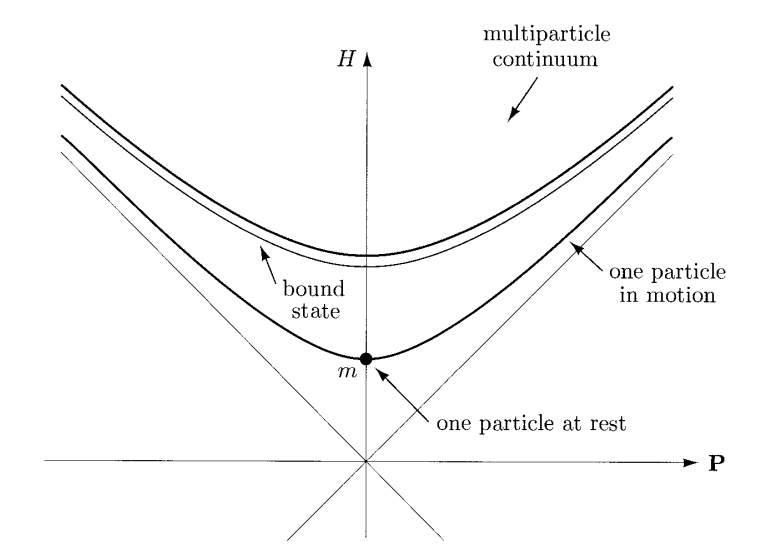
\includegraphics[height=8.10cm ,width=12.02cm]{QFT1/FSR1.png}
\caption{Particle's energy-momentum relation}
\end{figure}
\\
Assume for now $x^0 > y^0$ and define $\langle \Omega | \phi(x) \phi(y) | \Omega \rangle_{C} = \langle \Omega | \phi(x) \phi(y) | \Omega \rangle - \langle \Omega | \phi(x)| \Omega \rangle \langle \Omega | \phi(y) | \Omega \rangle$ as connected two point function. (The term $\langle \Omega | \phi(x)| \Omega \rangle \langle | \Omega \phi(y) | \Omega \rangle$ is usually zero by symmetry; for higher spin fields, it is zero by Lorentz invariance.) The connected two point function is
\[\langle \Omega | \phi(x) \phi(y) | \Omega \rangle_{C} = \sum_{\lambda} \int \frac{d^3p}{(2\pi)^3} \frac{1}{2E_{\bm{p}}} \langle \Omega | \phi(x) |\lambda_{\bm{p}}\rangle\langle\lambda_{\bm{p}}| \phi(y) | \Omega \rangle\]
It can be verified that
\[\langle \Omega | \phi(x) |\lambda_{\bm{p}}\rangle = \langle \Omega | \phi(0) | \lambda_0 \rangle e^{ipx} |_{p^0 = E_{\bm{p}}}\]
So,
\[\langle \Omega | \phi(x) \phi(y) | \Omega \rangle_C = \sum_{\lambda} \int \frac{d^4p}{(2\pi)^4} \frac{-i}{p^2 + m_{\lambda}^2 -i\epsilon} e^{ip(x-y)} |\langle \Omega | \phi(0) | \lambda_0 \rangle|^2\]
Analogous expressions hold for the case $y^0 > x^0$, and both cases can be summarized as
\[\langle \Omega | T \phi(x) \phi(y) | \Omega \rangle_C = \int_0^{\infty} \frac{dM^2}{2\pi} \rho(M^2) D_F(x-y;M^2)\]
and 
\[\rho(M^2) = \sum_{\lambda} (2\pi) \delta(M^2-m^2)|\langle \Omega | \phi(0) | \lambda_0 \rangle|^2 \]
\begin{figure}[!h]
\centering
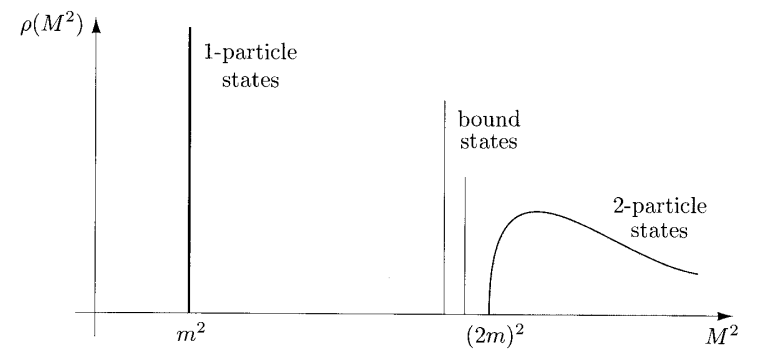
\includegraphics[height=5.33cm ,width=13.26cm]{QFT1/FSR2.png}
\caption{The structure of the spectral density function $\rho(M^2)$}
\end{figure}\\
The one-particle state contribute an isolated delta function to the spectral density function, so
\[\rho(M^2) = 2\pi \delta (M^2 -m^2) \cdot Z + \mbox{ (nothing else until $M^2 > \sim (2m)^2$) }\]
$Z = |\langle \Omega | \phi(0) | \lambda_0 \rangle|^2$ is called field-strength renormalization. $m$ is the physical mass of a single particle of the $\phi$ boson. The Fourier transformation of the two point function is
\begin{eqnarray}
&\phantom{=}& \int d^4x e^{-ipx} \langle \Omega | T \phi(x) \phi(0) | \Omega \rangle_C \nonumber \\  
&=& \int_{0}^{\infty} \frac{dM^2}{2\pi} \rho(M^2) \frac{-i}{p^2+M^2-i\epsilon} = \frac{-iZ}{p^2+m^2-i\epsilon} +  \int_{\sim 4m^2}^{\infty} \frac{dM^2}{2\pi} \rho(M^2) \frac{-i}{p^2+M^2-i\epsilon} \nonumber
\end{eqnarray}
\begin{figure}[!h]
\centering
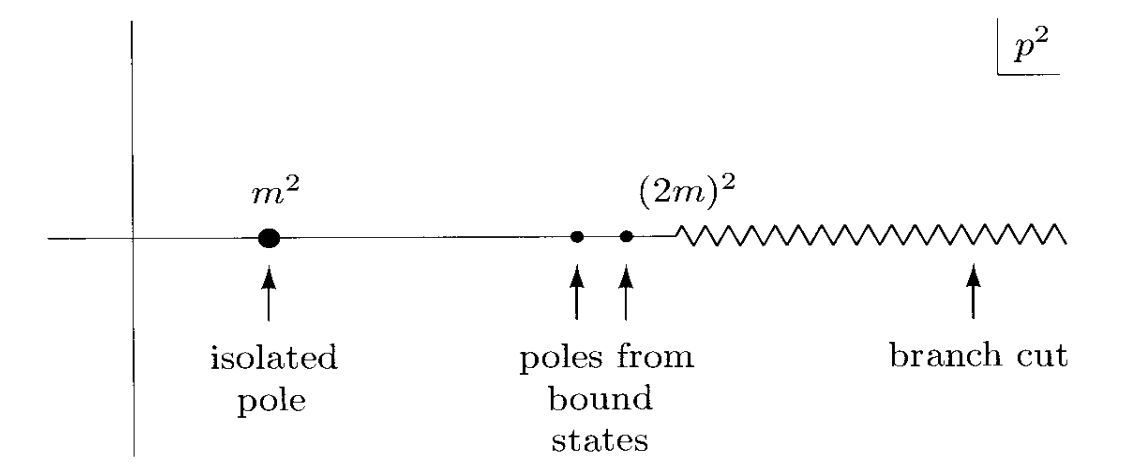
\includegraphics[height=4.73cm ,width=11.22cm]{QFT1/FSR3.png}
\caption{The structure of the two point function in Fourier space}
\end{figure}
\vspace{80pt}

\subsection{LSZ reduction formula}
\begin{newthem}[LSZ reduction formula]
\begin{eqnarray}
&& \quad \prod_1^n \int d^4 x_i e^{-ip_ix_i} \prod_1^m d^4 y_j e^{ik_jy_j} \langle \Omega | T \{\phi(x_1) \cdots \phi(x_n) \phi(y_1) \cdots \phi(y_m)\} | \Omega \rangle \nonumber \\
&& \underset{ p_i^0 \to E_{\bm{p}_i}\, k_i^0 \to E_{\bm{k}_i}}{\sim}  \left( \prod_1^n \frac{-\sqrt{Z} i}{p_i^2 + m^2 -i\epsilon} \right) \left( \prod_1^m \frac{-\sqrt{Z} i}{k_i^2 + m^2 -i\epsilon} \right) \langle \bm{p}_1 \cdots \bm{p}_n | S | \bm{k}_1 \cdots \bm{k}_m \rangle \nonumber
\end{eqnarray}
\end{newthem}
\noindent
The $\sim$ means the two sides of the expression share the same singular structure around $p_i^0 \to E_{\bm{p}_i}$, $k_i^0 \to E_{\bm{k}_i}$.
The proof can be found in chapter 7.2 of \emph{An introduction to quantum field theory (M.E.Peskin \& D.V.Schroeder)}.
To express the formula above in the language of Feynman diagrams, we consider the S-matrix element for 2-particle $\to$ 2-particle for example. Note the disconnected diagram should be disregarded because they do not have the singularity structure with a product of four poles indicated by on the right side of the LSZ reduction formula. So, the exact four point function
\[\prod_1^2 \int d^4 x_i e^{-ip_ix_i} \prod_1^2 d^4 y_i e^{ik_jy_j} \langle \Omega | T \{\phi(x_1)\phi(x_2)\phi(y_1) \phi(y_2)\} | \Omega \rangle \]
has the general form showed as below.
\begin{figure}[!h]
\centering
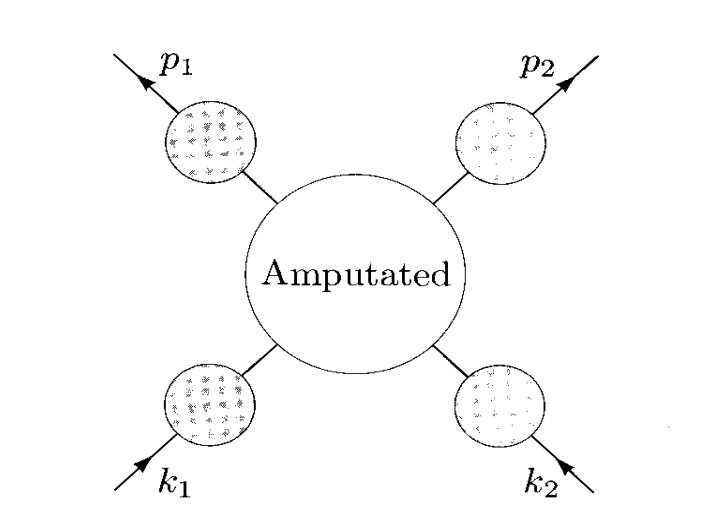
\includegraphics[height=5.26cm ,width=7.07cm]{QFT1/LSZ1.png}
\caption{Amputated Feynman diagram}
\end{figure}\\
We can sum up the corrections to each external leg. Let $-iM^2(p^2)$ denote the sum of all 1PI insertions into the scalar propagator:
\begin{figure}[!h]
\centering
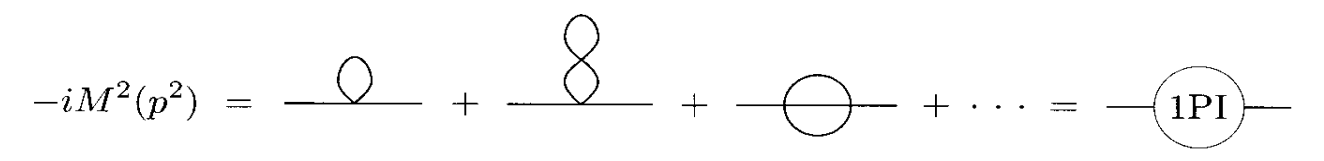
\includegraphics[height=1.61cm ,width=13.24cm]{QFT1/LSZ2.png}
\caption{Diagram representation of 1PI propagator}
\end{figure}
\begin{note}
One-particle-irreducible, or 1PI for short, refers to diagrams that is still connected after one line is cut
\end{note}
\noindent
Then the exact propagator can be written as a geometric series in
Figure 21.9.
\begin{figure}[!h]
\centering
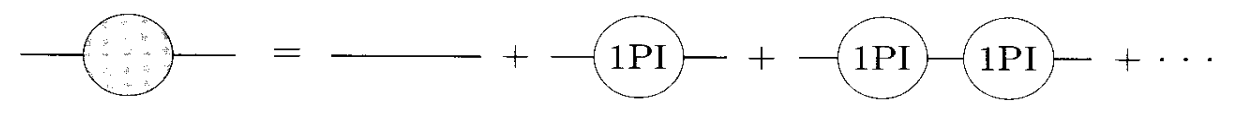
\includegraphics[height=1.17cm ,width=12.44cm]{QFT1/LSZ3.png}
\caption{Diagram representation of exact propagator}
\end{figure}\\
The result is $\frac{-i}{p^2 + m_0^2 + M^2}$. If we expand each resummed propagator about the physical particle pole, we see that each external leg of the four-point amplitude contributes
\[\frac{-i}{p^2 + m_0^2 + M^2} \underset{p^0 \to E_{\bm{p}}}{\sim} \frac{-iZ}{p^2+m^2} + \mbox{ (regular) }\]
Thus, the sum of diagrams contains a product of four point poles:
\[\frac{-iZ}{p_1^2 + m^2} \frac{-iZ}{p_2^2 + m^2} \frac{-iZ}{k_1^2 + m^2} \frac{-iZ}{k_2^2 + m^2}\]
So, the S matrix element can be represented by 
\begin{figure}[!h]
\centering
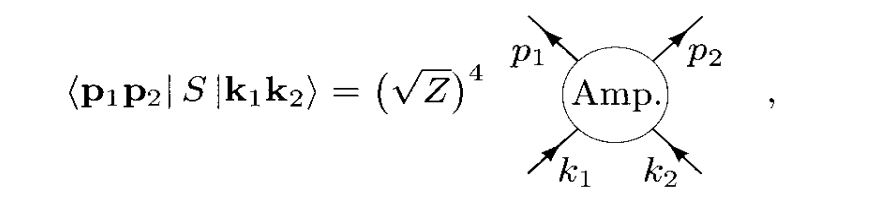
\includegraphics[height=2.04cm ,width=8.75cm]{QFT1/LSZ4.png}
\caption{Feynman diagram representation of LSZ reduction formula}
\end{figure}\\
It is easy to be generalized to the more complicated scattering cases. After Fourier transforming the n-point function to momentum space and cutting off the external legs, the Feynman rules for S-matrix element can be stated as follows:
\begin{enumerate}
\item For each propagator, $P = \frac{-i}{p^2 + m_0^2 -i\epsilon}$;
\item For each vertex, $V = -i\lambda_0$;
\item For each external point, $E=1$;
\item Impose momentum conservation at each vertex;
\item Integrate over each undetermined loop momentum: $\int \frac{d^4p}{(2\pi)^4}$;
\item Divided by the symmetry factor;
\item Multiply the total momentum conservation factor $(2\pi)^4 \delta(\sum p_f - \sum p_i)$ 
\end{enumerate}
We can write $\langle f | S | i \rangle = (Z_1)^{\frac{n_s}{2}} i \mathcal{M} (2\pi)^4 \delta(\sum p_f - \sum p_i)$ for convenience.

\section{Renormalization}
\noindent
Renormalization, the procedure in quantum field theory by which divergent parts of a calculation, leading to nonsensical infinite results, are absorbed by redefinition into a few measurable quantities, so yielding finite answers.

\subsection{Counting of ultraviolet divergence}
\noindent
Consider a pure scalar theory in $d$ dimensions with a $\phi^n$ interaction term
\[\mathcal{L} = -\frac{1}{2} \partial^{\mu} \phi \partial_{\mu} \phi -\frac{1}{2}m^2 \phi^2 - \frac{\lambda}{n!}\phi^n\]
Let $N$ be the number of external lines in the diagram, $P$ the number of propagators, $V$ the number of vertices. The number of the loops in the diagram is $L=P-V+1$.  There are $n$ lines meeting at each vertex, so $nV = 2P+N$. Loosely speaking, each loop has an integral $d^d p$, each propagator has a factor $p^{-2}$, so the superficial degrees of divergence is
\[D = dL - 2P = d + [n(\frac{d-2}{2})-d)]V - (\frac{d-2}{2})N\]
According the superficial degrees of divergence of the diagram. These three possible types of ultraviolet behaviour of quantum field theories. We will refer to them as follows

\begin{enumerate}
\item Super-renormalizable theory: Only a finite number of Feynman diagrams superficially diverge.
\item renormalizable theory: Only a finite number of amplitudes superficially diverge; however, divergences
occur at all orders in perturbation theory. 
\item Non-renormalizable theory: All amplitudes are divergent at a sufficiently high order in perturbation
theory.
\end{enumerate}
\noindent
So, for $\phi^4$ theory in four dimension, $D = 4 - N$. It is a renormalizable theory. For $\phi^3$ theory in four dimension, $D = 4 - V -N$. It is a super-renormalizable theory. For $\phi^6$ theory in four dimension, $D = 4 + 2V -N$. It is a Non-renormalizable theory. \\ \\
The superficial degrees of freedom can also be derived from dimensional analysis. The dimension of $\lambda$ is $d - \frac{n(d-2)}{2}$. Now consider an arbitrary diagram with $N$ external lines. One way that such a diagram could arise is from an interaction term $\eta \phi^N$ in the Lagrangian. The dimension of $\eta$ would then be $d - \frac{N(d-2)}{2}$, and therefore we conclude that any (amputated) diagram with $N$ external lines has dimension $d - \frac{N(d-2)}{2}$. In our theory with only the $\lambda \phi^n$ vertex, if the diagram has $V$ vertices, its divergent part is proportional to $\lambda^V \Lambda^D$, where $\Lambda$ is a high momentum cut-off and $D$ is the superficial degree of divergence.  Applying dimensional analysis, we find
\[d - \frac{N(d-2)}{2} = V[d - \frac{n(d-2)}{2}] + D\]
Note that the quantity that multiplies $V$ in this expression is just the dimension of the coupling constant $\lambda$. Thus we can characterize the three degrees of renormalizability in a second way:

\begin{enumerate}
\item Super-renormalizable: Coupling constant has positive mass dimension.
\item  renormalizable: Coupling constant is dimensionless.
\item  Non-renormalizable: Coupling constant has negative mass dimension.
\end{enumerate}

\subsection{Renormalized perturbation theory}
The Lagrangian of $\phi^4$ theory is 
\[\mathcal{L} = -\frac{1}{2} \partial^{\mu} \phi \partial_{\mu} \phi -\frac{1}{2}m_0^2 \phi^2 - \frac{\lambda_0}{4!}\phi^4\]
\\
We write $m_0$ and $\lambda_0$, to emphasize that these are the bare values of the mass and coupling constant, not the values measured in experiments.
Since the theory is invariant under $\phi \to -\phi$, all amplitudes with an odd number of external legs vanish. The only divergent amplitudes are therefore
\begin{figure}[!h]
\centering
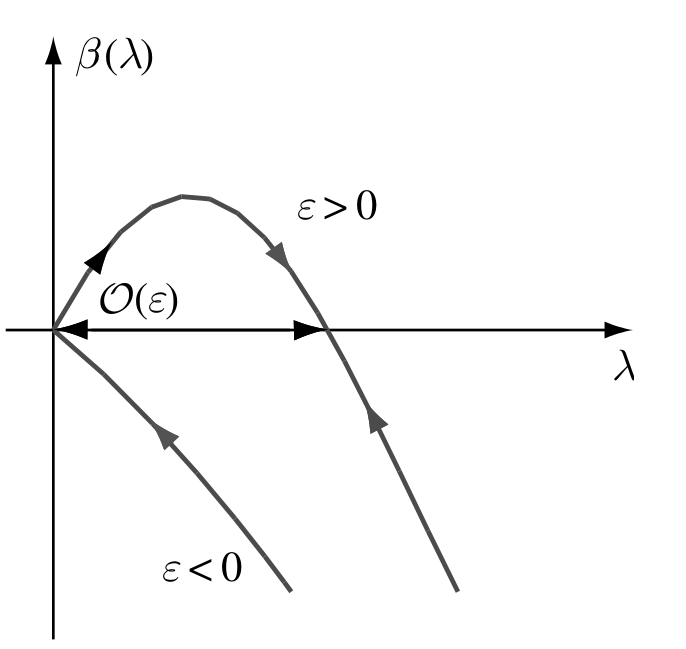
\includegraphics[height=4cm ,width=8.89cm]{QFT1/RG1.png}
\caption{Divergence of $\phi^4$ theory}
\end{figure}
\noindent
Ignoring the vacuum diagram, these amplitudes contain three infinite constants. Our goal is to absorb these constants into the three unobservable parameters of the theory: the bare mass, the bare coupling constant, and the field strength. To accomplish this goal, it is convenient to reformulate the perturbation expansion so that these unobservable quantities do not appear
explicitly in the Feynman rules. Recall that the exact two-point function has the form
\[\int d^4x \langle \Omega | \phi(x) \phi(0) | \Omega \rangle e^{-ipx} = \frac{-iZ}{p^2+m^2} + \mbox{ terms regular at } p^2 = m^2\]
We can eliminate the $Z$ from this equation by rescaling the field:
$\phi = Z^{\frac{1}{2}} \phi_r$
We also define
\[\delta_Z = Z -1 \quad \delta_m = Zm_0^2 - m^2 \quad \delta_{\lambda} = \lambda_0 Z^2 - \lambda\]
Then the Lagrangian becomes
\[\mathcal{L} = -\frac{1}{2} \partial^{\mu} \phi_r \partial_{\mu} \phi_r -\frac{1}{2}m^2 \phi_r^2 - \frac{\lambda}{4!}\phi_r^4 -\frac{1}{2} \delta_Z \partial^{\mu} \phi_r \partial_{\mu} \phi_r -\frac{1}{2}\delta_m \phi_r^2 - \frac{\delta \lambda}{4!}\phi_r^4\]
The last three terms, known as counter-terms, have absorbed the infinite but unobservable shifts between the bare parameters and the physical parameters.We give precise definitions of the physical mass and coupling constant as Figure 21.12.\\
\begin{figure}[!h]
\centering
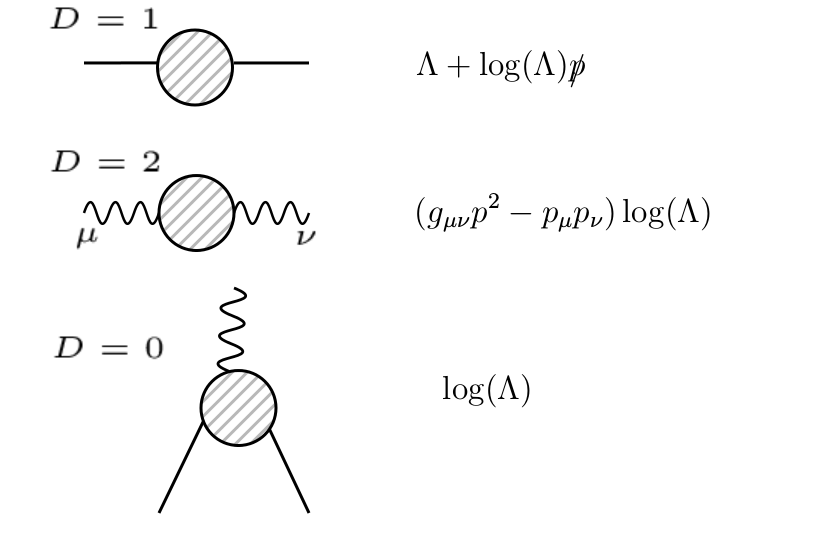
\includegraphics[height=3cm ,width=11.25cm]{QFT1/RG2.png}
\caption{Renormalization condition}
\end{figure}

\noindent
The renormalization scheme here is called on-shell (OS) scheme. Other renormalization scheme would be introduced later.
These equations are called renormalization conditions.
Our new Lagrangian gives a new set of Feynman rules as Figure 21.13.
\begin{figure}[!h]
\centering
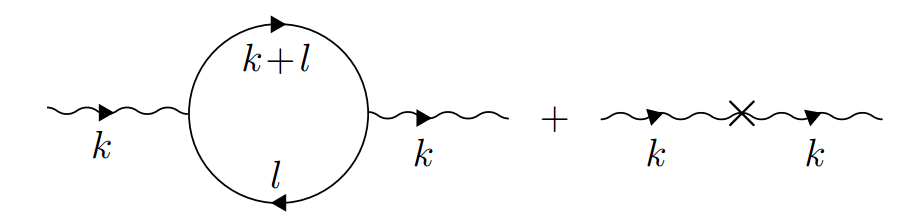
\includegraphics[height=6cm ,width=9cm]{QFT1/RG3.png}
\caption{Feynman rules for renormalized perturbation theory}
\end{figure}

\noindent
We can use these new Feynman rules to compute any amplitude in $\phi^4$ theory. The procedure is as follows. Compute the desired amplitude as the sum of all possible diagrams created from the propagator and vertices shown above. The loop integrals in the diagrams will often diverge, so one must introduce a regulator. The result of this computation will be a function of the three unknown parameters $\delta_Z$, $\delta_m$, and $\delta_{\lambda}$. Adjust ( or "renormalise") these three parameters as necessary to maintain the renormalization conditions. After this adjustment, the expression for the amplitude should be finite and independent of the regulator.
\\
This procedure, using Feynman rules with counter-terms, is known as renormalized perturbation theory. 

\subsubsection{Mandelstam variable}
In theoretical physics, the \href{https://en.wikipedia.org/wiki/Mandelstam_variables}{\textbf{Mandelstam variable}}  are numerical quantities that encode the energy, momentum, and angles of particles in a scattering process in a Lorentz-invariant fashion. They are used for scattering processes of two particles to two particles. 
The Mandelstam variables $s$, $t$, $u$ are then defined by
\begin{eqnarray}
s=-(p_{1}+p_{2})^{2}=-(p_{3}+p_{4})^{2} \nonumber \\
t=-(p_{1}-p_{3})^{2}=-(p_{2}-p_{4})^{2} \nonumber \\
u=-(p_{1}-p_{4})^{2}=-(p_{2}-p_{3})^{2} \nonumber
\end{eqnarray}
\\
Where $p_1$ and $p_2$ are the four-momenta of the incoming particles and $p_3$ and $p_4$ are the four-momenta of the outgoing particles.
$s$ is also known as the square of the center-of-mass energy (invariant mass) and $t$ is also known as the square of the four-momentum transfer.\\
We can verify that
\[s+t+u = m_1^2 + m_3^2 + m_3^2 +m_4^2\]

\subsection{Techniques for renormalization}
\subsubsection{Feynman's formula}
\begin{newthem}[Feynman's formula]
\[ \frac{1}{A_1 \cdots A_n} = \int dF_n (x_1A_1+ \cdots +x_nA_n)^{-n}\]
where the integration measure over the Feynman parameters $x_i$ is
\[\int dF_n = (n-1)! \int_0^1 dx_1 \cdots dx_n \delta(x_1+\cdots+x_n-1)\]
This measure is normalized so that
\[\int dF_n = 1\]
A generalization of Feynman's formula is
\[ \frac{1}{A_1^{\alpha_1} \cdots A_n^{\alpha_n}} = \frac{\Gamma(\sum_i \alpha_i)}{\prod_i \Gamma(\alpha_i)} \frac{1}{(n-1)!}\int dF_n \frac{\prod_i x_i^{\alpha_i-1}}{(\sum_i x_i A_i)^{\sum_i \alpha_i}}\]
\end{newthem}
\begin{figure}[!h]
\centering
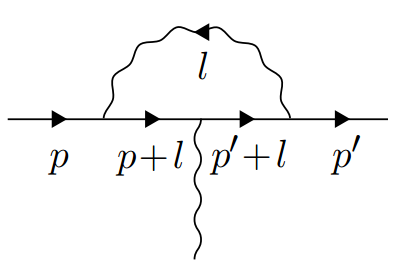
\includegraphics[height=4.41cm ,width=5.77cm]{QFT1/RG5.png}
\caption{Wick rotation}
\end{figure}

\subsubsection{Wick rotation}
For an integral $\int d^d q f(q^2-i\epsilon)$, if the integrand vanishes fast enough as $|q_0| \to \infty$, we can rotate this contour clockwise by $\frac{\pi}{2}$, so that it runs from $-i\infty$ to $i\infty$. In making this Wick rotation, the contour does not pass over any poles. (The $i\epsilon$ are needed to make this statement unambiguous.) Thus the value of the integral is unchanged. It is now convenient to define a Euclidean d-dimensional vector $\bar{q}$ via $q^0 = i \bar{q}_d$ and $q_j = \bar{q}_j$; then $q^2 = \bar{q}^2$, where
\[\bar{q}^2 = \bar{q}_1^2 + \cdots + \bar{q}_d^2\]
Also, $d^dq = id^d \bar{q}$.Therefore, in general,
\[\int d^d q f(q^2-i\epsilon) = i \int d^d\bar{q} f(\bar{q}^2)\]

\subsubsection{Dimensional regularization}
Dimensional regularization is a method for regularizing integrals in the evaluation of Feynman diagrams. For example, if one wishes to evaluate a loop integral which is logarithmically divergent in four dimensions, like
\[\int {\frac {d^{d}p}{(2\pi )^{d}}}{\frac {1}{\left(p^{2}+m^{2}\right)^{2}}}\]
\\
One first rewrites the integral in some way so that the number of variables integrated over does not depend on d, and then we formally vary the parameter $d$, to include non-integral values like $d=4-\epsilon$.
\[\int _{0}^{\infty }{\frac {dp}{(2\pi )^{4-\varepsilon }}}{\frac {2\pi ^{(4-\varepsilon )/2}}{\Gamma \left({\frac {4-\varepsilon }{2}}\right)}}{\frac {p^{3-\varepsilon }}{\left(p^{2}+m^{2}\right)^{2}}}={\frac {2^{\varepsilon -4}\pi ^{{\frac {\varepsilon }{2}}-1}}{\sin({\frac {\pi \varepsilon }{2}})\Gamma (1-{\frac {\varepsilon }{2}})}}m^{-\varepsilon }={\frac {1}{8\pi ^{2}\varepsilon }}-{\frac {1}{16\pi ^{2}}}\left(\ln {\frac {m^{2}}{4\pi }}+\gamma \right)+{\mathcal {O}}(\varepsilon )\]
There is a useful formula for calculating the integral
\[\int \frac{d^d \bar{q}}{(2\pi)^{d}} \frac{(\bar{q}^2)^a}{(\bar{q}^2+D)^b} = \frac{\Gamma(b-a-\frac{1}{2}d) \Gamma(a+\frac{1}{2}d)}{(4\pi)^{d/2} \Gamma(b) \Gamma(\frac{1}{2}d)} D^{-(b-a-d/2)}\]
If $a=0$, then the formula will be
\[\int \frac{d^d \bar{q}}{(2\pi)^{d}} \frac{1}{(\bar{q}^2+D)^b} = \frac{\Gamma(b-\frac{1}{2}d)}{(4\pi)^{d/2} \Gamma(b)} D^{-(b-d/2)}\]

\subsection{One loop structure of $\phi^4$ theory}
First consider the basic two-particle scattering amplitude,
\begin{figure}[!h]
\centering
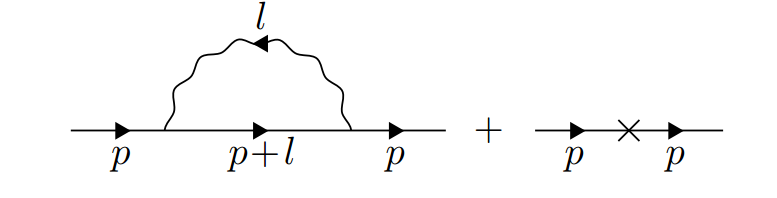
\includegraphics[height=3.71cm ,width=12.65cm]{QFT1/RG4.png}
\caption{Feynman diagram representation of two-particle scattering to one loop}
\end{figure}
If we define $p = p_1 + p_2$, then the second diagram of Figure 21.15 is
\[\frac{(-i\lambda)^2}{2} \int \frac{d^4k}{(2\pi)^4} \frac{-i}{k^2+m^2} \frac{-i}{(k+p)^2+m^2} \equiv (-i\lambda)^2 iV(-p^2)\]
So the entire amplitude is therefore
\[i\mathcal{M} = -i\lambda + (-i\lambda)^2 [iV(s) + iV(t) + iV(u)] -i\delta_{\lambda} + \mathcal{O}(\lambda^3)\] 
To keep $\lambda$ dimensionless in dimensional regularization, we can make the transformation $\lambda \to \lambda \tilde{\mu}^{\epsilon}$. Here, $\tilde{\mu}$ is an arbitrary number with mass dimension 1 and $\epsilon \equiv 4-d$. 
\\
We can calculate that
\[V(-p^2) = -\frac{1}{32\pi^2} \int_0^1 (\frac{2}{\epsilon} + \ln(\frac{\mu^2}{D(-p^2)}))\]
where $\mu \equiv  \sqrt{4\pi} e^{-\gamma/2} \tilde{\mu}$, $D(-p^2) = x(1-x)p^2+m^2$
\\
The renormalization condition implies that
\[\delta_{\lambda} = -\lambda^2[V(4m^2)+2V(0)] + \mathcal{O}(\lambda^3)\]
So,
\[i\mathcal{M} = -i\lambda -\frac{i\lambda^2}{32\pi^2} \int_0^1 dx \left[\ln(\frac{D(s)}{D(4m^2)}) +\ln(\frac{D(t)}{D(0)})+\ln(\frac{D(u)}{D(0)})\right] + \mathcal{O}(\lambda^3)\]
To determine $\delta_Z$ and $\delta_m$ we must compute the two-point function. Define $-iM(p^2)$ as the sum of all one-particle-irreducible insertions into the propagator.The full two-point function is given by
\[\frac{-i}{p^2 + m^2 + M^2}\]
The renormalization conditions require that the pole in this full propagator occur at $p^2=-m^2$ and have residue $1$. These two conditions are equivalent, respectively, to
\[M^2(p^2)|_{p^2=-m^2} = 0 \quad \left. \frac{d}{dp^2} M^2(p^2)\right|_{p^2=-m^2} =0\]
We can calculate that
\[-iM^2(p^2) = \frac{i\lambda}{32\pi^2}(\frac{2}{\epsilon} + \ln(\frac{\mu^2}{m^2})+1)m^2 -i(p^2\delta_Z + \delta_m)\]
So, to the order of $\lambda$, 
\[\delta_Z=\mathcal{O}(\lambda^2) \quad \delta_m = \frac{\lambda}{32\pi^2}(\frac{2}{\epsilon} + \ln(\frac{\mu^2}{m^2})+1)m^2 + \mathcal{O}(\lambda^2) \quad M^2(p^2) =\mathcal{O}(\lambda^2)\]
\\
The detailed calculation can be found in chapter 10.2 of \emph{An introduction to quantum field theory (M.E.Peskin \& D.V.Schroeder)} and will be eliminated here.

\subsubsection{Perturbation theory to all orders}
We begin by summing all one-particle irreducible diagrams with two external lines; this gives us the self-energy $M^2$. We next sum all amputated diagrams with four external lines; this gives us the four-point vertex function $V_4(k_1, k_2, k_3, k_4)$. (We can prove that amputated diagrams with four external lines must be one-particle irreducible). Order by order in $\lambda$, we must adjust the value of the lagrangian coefficients $\delta_Z$, $\delta_m$, and $\delta_{\lambda}$ to maintain the conditions $M^2(-m^2) = 0$, $\frac{dM^2}{dp^2}(-m^2) = 0$, and $V_4(s=4m^2) =0$. 
\\
Next we will construct the n-point vertex functions $V_n$ with $4 < n \leq E$, where $E$ is the number of external lines in the process of interest. We compute these using a skeleton expansion. This means that we draw all the contributing 1PI diagrams, but omit diagrams that include either propagator or three-point vertex corrections. That is, we include only diagrams that are not only 1PI, but also 2PI and 4PI: they remain connected when any one, two, or four lines are cut. (Cutting four lines may isolate a single tree-level vertex, but nothing more complicated.) Then we take the propagators and vertices in these diagrams to be given by the exact propagator $\frac{-i}{p^2+m^2+M^2(p^2)}$ and vertex $V_4(k_1,k_2,k_3,k_4)$, rather than by the tree-level propagator and vertex. We then sum these skeleton diagrams to get $V_n$ for $4 < n \leq E$. Order by order in $\lambda$, this procedure is
equivalent to computing $V_n$ by summing the usual set of contributing 1PI diagrams.
\\
Next we draw all tree-level diagrams that contribute to the process of interest (which has $E$ external lines), including not only four-point vertices, but also n-point vertices. Then we evaluate these diagrams using the exact propagator for internal lines, and the exact 1PI vertices $V_n$; external lines are assigned a factor of one. We sum these tree diagrams to get the scattering amplitude. Order by order in $\lambda$, this procedure is equivalent to computing the scattering amplitude by summing the usual set of contributing diagrams.
\\
Thus we now know how to compute an arbitrary scattering amplitude
to arbitrarily high order. The procedure is the same in any quantum field theory; only the form of the propagators and vertices change, depending on the spins of the fields.

\subsection{General renormalization theory}
Recall some of the major results and methods of renormalization theory:
\begin{enumerate}
\item In perturbation theory, bare and physical quantities are related by ultraviolet-divergent expressions
\[m_{phys} = m_0 + \Delta_m\]
where $m_{phys}$ is finite, $\Delta_m$ is ultraviolet-divergent, and so $m_0$ is necessarily ultraviolet-divergent.
\item We express the Lagrangian in terms of physical quantites, and separate it into
\[\mathcal{L} = \mathcal{L}_0 + \mathcal{L}_I + \mathcal{L}_{CT}\]
where $\mathcal{L}_0$ is the canonically normalized free Lagrangian for physical fields and masses, $\mathcal{L}_I$ contains the interaction, again in terms of physical parameters, and $\mathcal{L}_{CT}$ contains the counterterms with ultraviolet divergent coefficients. From $\mathcal{L}_0$, we obtain the propagators of the physical fields. $\mathcal{L}_I$ and $\mathcal{L}_{CT}$ give
interaction vertices.
\item At the one-loop level, the self-energy is given by the effective two-point vertices: the 1PI two-point vertex of the interaction and the counter-term two-point vertex. The counterterms absorb ultraviolet divergences, and the finite parts of the counterterms are determined by renormalization conditions,
which ensure the quantities in $\mathcal{L}_0 + \mathcal{L}_I$ are physical. The conditions constrain the self-energy and the effective vertices, and give a finite, uniquely-determined value for the counterterms.
\end{enumerate}
\subsubsection{Degrees of divergences}
Now, for a general theory in $d$ spacetime dimensions, the field content is given by $\phi_f$, $f=1,2,\cdots$, where $f$ labels
the field type. $[\phi_f]=\Delta f$ and $\Delta f$ in all physical theories. We have interaction vertices of type $i$, $i = 1,2,\cdots$
contributing a term of the form
\[\lambda_i \partial^{n_i} \prod_f \phi_f^{n_{if}}\]
Here, $\lambda_i$ is the coupling constant, with dimension
\[[\lambda_i] = \kappa_i = d - n_i - \sum_f n_{if}\Delta f \]
Now consider a 1PI diagram in such a theory:
\[E_f \equiv \mbox{ number of external lines of } \phi_f\]
\[V_i \equiv \mbox{ number of vertices of type i }.\]
Then $M \sim \Lambda^D \prod_i \lambda_i ^{V_i}$ and so $D = [M] - \sum_i V_i \kappa_i$. Again
\[[M] - d = -\sum E_f \Delta f\]
and so the general expression for the superficial degree of divergence is given by
\[D = d - \sum_f E_f \Delta f - \sum_i V_i \kappa_i\]
Diagrams which are ultraviolet divergent satisfy
\[\sum_f E_f \Delta f + \sum_i V_i \kappa_i < d\]
We can now divide all theories into
\begin{enumerate}
\item All $\kappa_i > 0$: superrenormalizable theories.
\item All $\kappa_i \geq 0$: renormalizable theories.
\item There exists at least one $\delta_i < 0$: non-renormalizable theories.
\end{enumerate}
These terms also apply to individual interactions for a vertex of type $i$:
\begin{enumerate}
\item $\kappa_i > 0$: super-renormalizable, relevant interaction.
\item $\kappa_i \geq 0$ : renormalizable, marginal interaction.
\item $\kappa_i < 0$: non-renormalizable, irrelevant interaction.
\end{enumerate}

\subsubsection{Cancellation of divergences}
Consider a generic divergent diagram $M$ of degree $D$; that is,
\[M = \int^{\Lambda} ds s^{D-1}\]
if all loop momenta are taken proportional to $s$. Generically, internal propagators have the form
\[\frac{1}{(as+p)^{\alpha}\cdots} \sim \frac{1}{s^{\alpha}}\]
for large $s$, where $a$ is a numerical constant and $p$ is a combination of the external momenta. Differentiating M,
with respect to $p$, $n$ times gives a term proportional to
\[\frac{1}{(as+p)^{\alpha+n}} \sim \frac{1}{s^{\alpha + n}} \]
and so $D+1$ derivatives with respect to the external momenta will make $M$ finite. This means that
\[M(p) = M_0 + M_1 p + \cdots + M_D p^D + \mbox{ finite terms}\]
where the argument $p$ of the function represents the collection of external momenta, we have suppressed the index structure, and $M_0,M_1,\cdots,M_D$ are potentially divergent constants. Suppose that $M$ has $E_f$ external lines of the field $\phi_f$. Then divergences of $M(p)$ can be cancelled by counterterms of the form
\[\sum_{j=0}^D A_j (\partial)^j \prod_f \phi_f^{E_f}\]
where the $A_j$ are divergent coefficients in order to cancel divergences in $M_j$. The index structure in $A_j \partial^j$ should
match the suppressed index structure of $M(p)$.

\section{Renormalization group}
\subsection{Modified minimal-subtraction scheme}
The Lagrangian of $\phi^4$ theory is
\[\mathcal{L} = -\frac{1}{2} \partial^{\mu} \phi \partial_{\mu} \phi -\frac{1}{2}m^2 \phi^2 - \frac{\lambda}{4!}\phi^4 -\frac{1}{2} \delta_Z \partial^{\mu} \phi \partial_{\mu} \phi -\frac{1}{2}\delta_m \phi_r - \frac{\delta \lambda}{4!}\phi^4\]
\\
For minimal-subtraction scheme, we do not demand that $m$ be the physics mass of the field and $\phi$  create a normalized one-particle state. The physical meaning of $\lambda$ is not expressed directly as well. Instead we choose $\delta_Z$, $\delta_m$ and $\delta_{\lambda}$ to cancel the infinities, and nothing more;
we say that $\delta_Z$, $\delta_m$ and $\delta_{\lambda}$ have no finite parts. It is called the modified minimal-subtraction or $\mathrm{\overline{MS}}$ scheme. ("modified" because we introduced $\mu$ via  $\lambda \to \lambda \tilde{\mu}^{\epsilon}$, with $\mu \equiv  \sqrt{4\pi} e^{-\gamma/2} \tilde{\mu}$; had we set $\mu = \tilde{\mu}$ instead, the scheme would be just plain minimal subtraction or MS.)
\\
For loop corrections to propagator,
\[\delta_Z=\mathcal{O}(\lambda^2) \quad \delta_m = \left[ \frac{\lambda}{16\pi^2} + \mathcal{O}(\lambda^2) \right]\frac{1}{\epsilon}m^2 \quad M^2(p^2) = \frac{\lambda}{32\pi^2}( \ln(\frac{m^2}{\mu^2})-1)m^2 + \mathcal{O}(\lambda^2)\]
\\
Firstly, in the $\mathrm{\overline{MS}}$ scheme, the propagator will no longer have a pole at $k^2=-m^2$. The pole will be somewhere else. However, by definition, the actual physical mass $m_{ph}$ of the particle is determined by the location of this pole: $k^2 = -m_{ph}^2$. Thus, the Lagrangian parameter $m$ is no longer the same as $m_{ph}$. The relation of $m$ and $m_{ph}$ is 
\[m_{ph}^2 = M^2(-m_{ph}^2) + m^2\]
To the lowest order, 
\[m_{ph}^2 = \left[1+\frac{\lambda}{32\pi^2}( \ln(\frac{m^2}{\mu^2})-1)\right] m^2\]
Because $m_{ph}$ is a independent of $\mu$, according to $\frac{d}{d\mu} m_{ph} = 0$, it can be derived that
\[\frac{dm}{d\ln \mu} = \left[\frac{\lambda}{32\pi^2}+\mathcal{O}(\lambda^2)\right] m\]
Furthermore, the residue of this pole is no longer one. Let us call the residue $R$. So, in the LSZ formula, we get a net factor of $\sqrt{R}$ for each external line when using the $\mathrm{\overline{MS}}$ scheme. And in $\phi^4$ theory,
\[R = 1 + \mathcal{O}(\lambda^2)\]
For loop corrections to vertex,
\[\delta_{\lambda} = \left[\frac{3\lambda^2}{16\pi^2} + \mathcal{O}(\lambda^3)\right]\frac{1}{\epsilon}\]
\[i\mathcal{M} = -i\lambda -\frac{i\lambda^2}{32\pi^2} \int_0^1 dx \left[\ln(\frac{D(s)}{\mu^2}) +\ln(\frac{D(t)}{\mu^2})+\ln(\frac{D(u)}{\mu^2})\right] + \mathcal{O}(\lambda^3)\]
For a process with $p^2 \gg m^2$, we have
\[ D \approx x(1-x)p^2\]
In OS renormalization scheme, the one-loop correction to propagator or vertex generally includes a factor
\[\ln \left( \frac{D}{D_0}\right ) \sim \ln \frac{p^2}{m^2}\]
so perturbation theory is no longer a good approximation when $p^2 \gg m^2$.
In $\overline{MS}$ renormalization scheme, introducing $\mu$ allows us to address this problem: if we choose $\mu \sim p$, no such logarithm arises. If we choose $\mu$ appropriately, that is, to be comparable to the momentum scale of the physical process, we can
improve our perturbation expansion. 
So $\lambda(\mu)$ and $m(\mu)$ can be considered as the scale-dependent coupling constants.
And the reason we get large logarithmic terms in the on-shell scheme is that we are trying to use coupling defined at one scale to describe physics at very different scales.

\subsection{Beta and gamma function}
\noindent
The Lagrangian of $\phi^4$ theory is 
\[\mathcal{L} = -\frac{1}{2} \partial^{\mu} \phi_0 \partial_{\mu} \phi_0 -\frac{1}{2}m_0^2 \phi_0^2 - \frac{\lambda_0}{4!}\phi_0^4\]
It can be written as
\[\mathcal{L} = -\frac{1}{2}Z_{\phi} \partial^{\mu} \phi \partial_{\mu} \phi -\frac{1}{2}Z_{m}m^2 \phi^2 - Z_{\lambda} \tilde{\mu}^{\epsilon}\frac{\lambda}{4!}\phi^4\]
So, 
\[\phi_0 = Z_{\phi}^{1/2}\phi \quad m_0 = Z_{\phi}^{-1/2} Z_{m}^{1/2}m \quad \lambda_0 = Z_{\phi}^{-2} Z_{\lambda} \lambda \tilde{\mu}^{\epsilon}\]
After using dimensional regularization, the infinities coming from loop integrals take the form of inverse powers of $\epsilon$. In the  $\mathrm{\overline{MS}}$ renormalization scheme, we choose the Zs to cancel off these powers of $1/\epsilon$, and nothing more. Therefore the Zs can be written as
\begin{eqnarray}
Z_{\phi} = 1 + \sum_{n=1}^{\infty} \frac{a_n(\lambda)}{\epsilon^n} \nonumber \\
Z_{m} = 1 + \sum_{n=1}^{\infty} \frac{b_n(\lambda)}{\epsilon^n} \nonumber \\
Z_{\lambda} = 1 + \sum_{n=1}^{\infty} \frac{c_n(\lambda)}{\epsilon^n} \nonumber 
\end{eqnarray}
In $\phi^4$ theory, $a_1 = \mathcal{O}(\lambda^2)$, $b_1 = \frac{\lambda}{16\pi^2} +  \mathcal{O}(\lambda^2)$,$c_1 = \frac{3\lambda}{16\pi^2} + \mathcal{O}(\lambda^2)$\\
Remember that bare fields and parameters must be independent of $\mu$.Define
\[G(\lambda,\epsilon) \equiv \ln(Z_{\phi}^{-2} Z_{\lambda}) = \sum_{n=1}^{\infty} \frac{G_n(\lambda)}{\epsilon^n}\]
We can calculate $G_1 = c_1 - 2a_1 = \frac{3\lambda}{16\pi^2} + \mathcal{O}(\lambda^2)$.
As $\ln \lambda_0 = G + \ln \lambda + \epsilon \ln \tilde{\mu} $. From the independence of $\lambda_0$, we can derive
\[\left ( 1 + \frac{\lambda G'_1}{\epsilon} + \cdots \right) \frac{d\lambda}{d\ln \mu} + \epsilon \lambda = 0\]
$\frac{d\lambda}{d\ln\mu}$ is the rate at which $\lambda$ must change to compensate for a small change in $\ln \mu$. If compensation is possible at all, this rate should be finite in the $\epsilon \to 0$ limit. In a renormalizable theory, we should have
\[\frac{d\lambda}{d\ln\mu} = -\epsilon\lambda + \beta(\lambda)\]
So
\[\beta(\lambda) = \lambda^2 G'_1(\lambda)\]
In $\phi^4$ theory, we have
\[\beta(\lambda) = \frac{3\lambda^2}{16\pi^2} + \mathcal{O}(\lambda^3)\]
Define
\[M(\lambda,\epsilon) \equiv \ln(Z_{m}^{1/2} Z_{\phi}^{-1/2}) = \sum_{n=1}^{\infty} \frac{M_n(\lambda)}{\epsilon^n}\]
We can calculate $M_1 = \frac{1}{2}b_1 - \frac{1}{2}a_1 = \frac{\lambda}{32\pi^2} + \mathcal{O}(\lambda^2)$.
As $\ln m_0 = M + \ln m $, define the anomalous dimension of the mass
\[\gamma_m(\lambda) \equiv \frac{1}{m} \frac{dm}{d \ln \mu}\]
From the independence of $m_0$, we can derive
\[\gamma_m(\lambda) = \lambda M'_1\]
In $\phi^4$ theory, we have
\[\gamma_m(\lambda) = \frac{\lambda}{32\pi^2} + \mathcal{O}(\lambda^2)\]
We can expand $\ln Z_{\phi}$ as
\[\ln Z_{\phi} = \frac{a_1}{\epsilon} + \cdots\]
Define the anomalous dimension of the field
\[\gamma_{\phi}(\lambda) \equiv \frac{1}{2} \frac{d\ln Z_{\phi}}{d \ln \mu}\]
We can derive
\[\gamma_{\phi}(\lambda) = -\frac{1}{2}\lambda a'_1\]
In $\phi^4$ theory, we have
\[\gamma_{\phi}(\lambda) = \mathcal{O}(\lambda^2)\]

\subsection{Callen-Symanzik equation}
Consider the $n$ point green function,
\[G^{(n)}(x_1,\cdots,x_n) \equiv \langle \Omega | T \phi(x_1) \cdots \phi(x_n) | \Omega \rangle_C \]
As $G^{(n)}_0 = Z_{\phi}^{n/2} G^{(n)}$, from the independence of bare Green's function, we have
\[\left( \frac{\partial}{\partial \ln \mu} + \beta(\lambda)  \frac{\partial}{\partial \lambda} + \gamma_m(\lambda) m  \frac{\partial}{\partial m} + n \gamma_{\phi}(\lambda)\right)G^{n}(x_1,\cdots,x_n;\lambda,m,\mu) = 0\]
\\
From now on, we will focus on the $\phi^4$ theory in massless limit. Firstly, consider the two point Green's function in momentum space $G^{(2)}(p)$, we can express its dependence on $p$ and $\mu$ as
\[G^{(2)} = \frac{-i}{p^2} g(-p^2/\mu^2,\lambda(\mu))\]
Then the C-S equation can be written as
\[\left[ p \frac{\partial}{\partial p} - \beta(\lambda)  \frac{\partial}{\partial \lambda} +2 - 2\gamma_{\phi}\right ] G^{(2)}(p,\lambda(\mu),\mu) = 0 \]
Here, $p \equiv (-p^2)^{1/2}$
In the free theory, $\beta$ and $\gamma$ vanish and we recover the trivial result
\[G^{(2)}(p) = \frac{-i}{p^2}\]
In an interacting theory, the solution to the C-S equation can be expressed as
\[G^{(2)}(p,\lambda_0,\mu_0) = G^{(2)}(\mu_0,\lambda_p,\mu_0)\exp \left (-\int_{p'=\mu_0}^{p'=p} d \ln(p'/\mu_0) \cdot 2[1-\gamma_{\phi}(\lambda_{p'})] \right )\]
Here, $\lambda_0 = \lambda(\mu_0)$, $\lambda_p$ satisfy the following equation
\[\frac{\partial}{\partial \ln p} \lambda_p(p,\lambda_0) = \beta(\lambda_p) \quad \lambda_p(\mu_0,\lambda_0) = \lambda_0\]
The solution can be checked directly by noticing that
\[\left ( p \frac{\partial}{\partial p} - \beta(\lambda_0) \frac{\partial}{\partial \lambda_0} \right ) \lambda_p(p,\lambda_0) = 0\]
A convenient way of writing the solution is
\[G^{(2)}(p,\lambda_0,\mu_0) =  \frac{-i}{p^2} g^{(2)}(\mu_0,\lambda_p,\mu_0)\exp \left (2\int_{\mu_0}^{p} d \ln(p'/\mu_0)  \gamma_{\phi}(\lambda_{p'}) \right )\]
And $g(\lambda_p) = 1 + O(\lambda_p^2)$
\\
Now consider the connected four-point function of $\phi^4$ theory evaluated at spacelike momenta $p_i$ such that $p_i^2= P^2$, $p_i \cdot p_j = 0$, so that $s$, $t$, and $u$ are of order $-P^2$. To leading order in perturbation theory, this function is given by
\[G^{(4)}(P) = \left (\frac{i}{P^2}\right )^4 (-i\lambda)\]
The solution of C-S equation is
\[G^{(4)}(p,\lambda_0,\mu_0) =  \frac{1}{P^8} g^{(4)}(\mu_0,\lambda_p,\mu_0)\exp \left (4\int_{\mu_0}^{p} d \ln(p'/\mu_0)  \gamma_{\phi}(\lambda_{p'}) \right )\]
And $g(\lambda_p) = -i\lambda_p + O(\lambda_p^2)$.
\\
The ordinary Feynman perturbation series for a Green's function depends both on the coupling constant $\lambda$ and on the dimensionless parameter $\ln(p^2/\mu_0^2)$. The perturbation theory can be badly behaved even when $\lambda$ is small if the ratio $p^2/\mu_0^2$ is large. The solutions of C-S equation reorganize this dependence into a function of the running coupling constant and an exponential scale factor. 
\\
The first factor of the solution is a function of the running coupling constant, evaluated at the momentum scale $p$. If $p$ were of order $\mu_0$, this function would essentially be the ordinary perturbation evaluation of the Green's function. We can make use of this same expression at the scale $p$, but to replace $\lambda_0$ with a new coupling constant $\lambda_p$ appropriate to that scale.
The exponential factor is the accumulated field strength rescaling of the correlation function from the reference point $\mu_0$ to the actual momentum $p$ at which the Green's function is evaluated. This factor receives a multiplicative contribution from each intermediate scale between $\mu$ and $p$.
\\
In $\phi^4$ theory, we have
\[\frac{d}{d\ln p} \lambda_p = \frac{3\lambda_p^2}{16\pi^2}\]
The solution is
\[\lambda_p = \frac{\lambda_0}{1 - \frac{3\lambda_0}{16\pi^2} \ln (p/\mu_0)}\]
This expression for the running coupling constant goes to zero at a logarithmic rate as $p \to 0$. If we expand the running coupling constant $\lambda_p$ in powers of $\lambda_0$, we find that the successive powers of the coupling constant are multiplied by powers of logarithms, 
\[\lambda_0^{n+1}(\ln p/\mu_0)^n\]
which become large and invalidate a simple perturbation expansion for $p$ much greater or much less than $\mu_0$. If the running coupling constant becomes large, as happens in $\phi^4$ theory for $p \to \infty$, the perturbation expansion will break down anyway, and we will need more advanced methods. However, if the running coupling constant becomes small, as for $\phi^4$ theory as $p \to 0$, we will have successfully organized the powers of logarithms into a meaningful and controlled expression.

\subsection{Running of coupling constants}
In the limit of $\epsilon \to 0$, the coupling constant satisfies the differential equation
\[\frac{\partial \lambda}{\partial \ln \mu} = \beta(\lambda)\]
Three behaviours are possible in the region of small $\lambda$:
\begin{enumerate}
\item $\beta(\lambda) > 0$
\item $\beta(\lambda) = 0$
\item $\beta(\lambda) < 0$
\end{enumerate}
\noindent
In theories of the first class, the running coupling constant goes to zero in the infra-red, leading to definite predictions about the small-momentum behaviour of the theory. However, the running coupling constant becomes large in the region of high momenta. Thus the short-distance behaviour of the theory cannot be computed using Feynman diagram perturbation theory.A Feynman diagram analysis is useful in such theories if one is mainly interested in large-distance or macroscopic behaviour.
\\
In theories of the second class, the coupling constant does not flow. In these theories, the running coupling constant is independent of the momentum scale, and thus equal to the bare coupling. This means that there can be no ultraviolet divergences in the relation of coupling constants. The only possible ultraviolet divergences in such theories are those associated with field rescaling, which automatically cancel in the computation of S-matrix elements. Such theories are called finite quantum field theories. Before the emergence of our modern understanding of renormalization, these theories would have been embraced as the solution to the problem of ultraviolet infinities. But in fact the known finite field theories in four dimensions are very special constructions the so-called gauge theories with extended supersymmetry with no known physical application. 
\\
In theories of the third class, the running coupling constant becomes large in the large-distance regime and becomes small at large momenta or short distances. Such theories are called asymptotically free. In theories of this class, the short-distance behaviour is completely solvable by Feynman diagram methods. Though ultraviolet divergences appear in every order of perturbation theory, the renormalization group tells us that the sum of these divergences is completely harmless.
\\
In the region of strong coupling, the approximation we have made, ignoring the higher-order terms in the $\beta$ function is no longer valid. It is a logical possibility that the leading order term is positive while the higher terms of the $\beta$ function are negative, so that the $\beta$ function has a zero at a non-zero value $\lambda_*$. When $\lambda_*$ approaches this value, the renormalization group flow slows to a halt; thus $\lambda = \lambda_*$ would be a non-trivial fixed point of the renormalization group. 
\\
If the $\beta$ function behaves in the vicinity of the fixed point as 
\[\beta \approx -B(\lambda - \lambda_*)\] 
where $B$ is a positive constant. For $\lambda$ near $\lambda_*$ 
\[\frac{d}{d\ln \mu} \lambda \approx -B(\lambda-\lambda_*)\]
The solution of this equation is
\[\lambda(\mu) = \lambda_* + C(\frac{\mu_0}{\mu})^B\]
Thus, $\lambda$ indeed tends to $\lambda_*$ as $\mu \to \infty$, and the rate of approach is governed by the slope of the $\beta$ function at the fixed point. The fixed point here is called ultraviolet-stable fixed point. 
\\
If $p$ is sufficiently large, $\lambda(p)$ is close to $\lambda_*$.In the massless limit, the solution of C-S equation for two point Green function in momentum space becomes
\[G^{(2)}(p,\lambda_0,\mu_0) \approx G^{(2)}(\mu_0,\lambda_*,\mu_0)\exp \left (- \ln(p/\mu_0) \cdot 2[1-\gamma_{\phi}(\lambda_*)] \right )\]
Thus the naive scaling law $G(p) \sim p^{-2}$ is changed to $G(p) \sim p^{-2[1-\gamma_{\phi}(\lambda_*)]}$. This has applications in the theory of critical phenomena.
\\
A similar behaviour is possible in an asymptotically free theory. If the $\beta$ function behaves in the vicinity of the fixed point as 
\[\beta \approx B(\lambda - \lambda_*)\] 
where $B$ is a positive constant.
the running coupling constant will tend to a fixed point as $\mu \to 0$.  The fixed point is called infrared-stable fixed points. 

\section{Spontaneous symmetry breaking}
\subsection{Effective action}
\[Z[J] = e^{-iE[J]} = \int \mathcal{D} \phi \exp\left[ i\int d^4x (\mathcal{L}[\phi] + J \phi) \right]\]
Define 
\[\phi_{\mathrm{cl}} (x) \equiv \langle \Omega | \phi(x) | \Omega \rangle_{J}\]
So, we can derive
\[\frac{\delta}{\delta J(x)} E[J] = - \phi_{\mathrm{cl}}(x)\]
Define effective action as
\[\Gamma[\phi_{\mathrm{cl}}] \equiv -E[J] - \int d^4y J(y) \phi_{\mathrm{cl}}(y)\]
Suppose $\mathcal{L}$ is invariant under transformation $U$, i.e. $\mathcal{L}(U\phi) = \mathcal{L}(\phi) $. Then we can prove than effective action $\Gamma$ is also invariant under transformation $U$, i.e. $\Gamma(U\phi_{\mathrm{cl}}) = \Gamma(\phi_{\mathrm{cl}}) $.

\begin{newproof}
\[ U\phi_{\mathrm{cl}}(x) = \langle \Omega | U\phi(x) | \Omega\rangle_{J} = \frac{\int \mathcal{D}\phi e^{i \int \mathcal{L}(\phi)+J\phi}U\phi(x)}{\int \mathcal{D}\phi e^{i \int \mathcal{L}(\phi)+J\phi}}\]
Define $J' = \frac{J\phi}{U\phi}$,  and we suppose the measure of path integral is invariant under transformation $U$, then we have
\[ U\phi_{\mathrm{cl}}(x) = \frac{\int \mathcal{D}U\phi e^{i \int \mathcal{L}(U\phi)+J'U\phi}U\phi(x)}{\int \mathcal{D}U\phi e^{i \int \mathcal{L}(U\phi)+J'U\phi}} =  \frac{\int \mathcal{D}\phi e^{i \int \mathcal{L}(\phi)+J'\phi}\phi(x)}{\int \mathcal{D}\phi e^{i \int \mathcal{L}(\phi)+J'\phi}} = \langle \Omega | \phi(x) | \Omega\rangle_{J'}\]
On the one hand, we have
\[\Gamma[U\phi_{\mathrm{cl}}] = E[J'] - \int d^4y J'(y)U\phi_{\mathrm{cl}}(y) =  E[J'] - \int d^4y J(y)\phi_{\mathrm{cl}}(y)\]
On the other hand, we have
\begin{eqnarray}
Z[J'] &=& \int \mathcal{D}\phi \exp \left[ i \int d^4x \mathcal{L}(\phi)+J'\phi \right] =  \int \mathcal{D}U\phi \exp \left[ i \int d^4x \mathcal{L}(U\phi)+J'U\phi \right] \nonumber
\\
&=& \int \mathcal{D}\phi \exp \left[ i \int d^4x \mathcal{L}(\phi)+J\phi \right] = Z[J] \nonumber
\end{eqnarray}
So, $\Gamma(U\phi_{\mathrm{cl}}) = \Gamma(\phi_{\mathrm{cl}})$.
\end{newproof}

\noindent
We can further verify that
\[\frac{\delta}{\delta \phi_{\mathrm{cl}}(x)} \Gamma[\phi_{\mathrm{cl}}] = -J(x)\]
If the external source is set to zero, the effective action satisfy the equation
\[\frac{\delta}{\delta \phi_{\mathrm{cl}}(x)} \Gamma[\phi_{\mathrm{cl}}] = 0\]
The solution to this equation are the values of $\langle \phi(x) \rangle$ in the stable quantum states of the theory. For a translational-invariant vacuum state, we will find a solution in which $\phi_{\mathrm{cl}}$ is independent of $x$. For simplicity, will assume the vacuum state in our following discussion are all translational-invariant. 
So, if $T$ is the time extent of the region and $V$ is its three dimensional volume, we can define the effective potential of the field by
\[\Gamma[\phi_{\mathrm{cl}}] = -(VT) \cdot V_{\mathrm{eff}}(\phi_{\mathrm{cl}})\]
The condition that $\Gamma[\phi_{\mathrm{cl}}]$ has an extreme then reduces to the simple equation
\[\frac{\partial}{\partial \phi_{\mathrm{cl}}} V_{\mathrm{eff}}(\phi_{\mathrm{cl}}) = 0\] 
A system with spontaneously broken symmetry will have several minimum of $V_{\mathrm{eff}}$, all with the same energy by virtue of the symmetry. The choice of one among these vacuum is the spontaneous symmetry breaking.

\subsection{Computation of the effective action}
\noindent
Decompose the Lagrangian into a piece depending on renormalized parameters and one containing the counter-terms
\[\mathcal{L} = \mathcal{L}_1 + \delta \mathcal{L}\]
Define $J_1$ by
\[\left. \frac{\delta \mathcal{L}_1}{\delta \phi} \right|_{\phi = \phi_{\mathrm{cl}}} + J_1(x) = 0\]
Define $\delta J$ by
\[J(x) = J_1(x) + \delta J(x)\]
So, we have
\[e^{-iE[J]} = \int \mathcal{D}\phi e^{i\int d^4x (\mathcal{L}_1 + J_1\phi)} e^{i\int d^4x (\delta \mathcal{L} + \delta J \phi)}\]
Replace $\phi$ by $\phi_{\mathrm{cl}}+\eta$,
\begin{eqnarray}
\int d^4x \, (\mathcal{L}_1 + J_1\phi) &=& \int d^4x \, (\mathcal{L}_1[\phi_{\mathrm{cl}}] + J_1\phi_{\mathrm{cl}}) + \int d^4x \, \eta(x) \left( \frac{\delta \mathcal{L}_1}{\delta \phi} + J_1 \right) \nonumber \\
&+& \frac{1}{2} \int d^4x \, d^4y \, \eta(x) \eta(y) \frac{\delta^2 \mathcal{L}_1}{\delta \phi(x) \delta \phi(y)} \nonumber \\
&+& \frac{1}{3!} \int d^4x \, d^4y \, d^4z \, \eta(x) \eta(y) \eta(z) \frac{\delta^3 \mathcal{L}_1}{\delta \phi(x) \delta \phi(y) \delta \phi(z)} + \cdots \nonumber
\end{eqnarray}
The term linear in $\eta$ vanishes by definition of $J_1$.  Keeping only the term up to quadratic order in $\eta$ and still neglecting the counter-terms, we have a pure Gaussian integral, which can be evaluated in terms of a functional determinant. Note that we might drop out the constant term  which is independent of  $\phi_{cl}$ and $J$, like $(2\pi i)^N$, in our derivation.
\begin{eqnarray}
&&\int \mathcal{D}\eta \exp \left[ i \left( \int ( \mathcal{L}_1 [\phi_{\mathrm{cl}}] + J_1\phi_{\mathrm{cl}} ) +  \frac{1}{2} \int \eta \frac{\delta^2 \mathcal{L}_1}{\delta \phi \delta \phi} \eta \right) \right] \nonumber \\
&=& \exp \left[ i \int ( \mathcal{L}_1 [\phi_{\mathrm{cl}}] + J_1\phi_{\mathrm{cl}} )\right] \left( \det \left[ - \frac{\delta^2 \mathcal{L}_1}{\delta \phi \delta \phi} \right] \right) ^{-\frac{1}{2}} \nonumber
\end{eqnarray}
Finally, put back the effects of the counter-term Lagrangian,writing it as
\[(\delta \mathcal{L}[\phi_{\mathrm{cl}}] + \delta J \phi_{\mathrm{cl}} ) + ( \delta \mathcal{L}[\phi_{\mathrm{cl}} + \eta] - \delta\mathcal{L} [\phi_{\mathrm{cl}}] + \delta J \eta)\]
Define
\[\mathcal{L}_2 = \left(\frac{1}{3!} \int d^4x \, d^4y \, d^4z \, \eta(x) \eta(y) \eta(z) \frac{\delta^3 \mathcal{L}_1}{\delta \phi(x) \delta \phi(y) \delta \phi(z)} + \cdots \right) + ( \delta \mathcal{L}[\phi_{\mathrm{cl}} + \eta] - \delta\mathcal{L} [\phi_{\mathrm{cl}}] + \delta J \eta)\]
So
\[e^{-iE[J]} = C_1 e^{i\int \mathcal{L}_2(\frac{1}{i} \frac{\delta}{\delta I})} \left. \int \mathcal{D}\eta e^{i\int \left(\frac{1}{2} \eta \frac{\delta^2 \mathcal{L}_1}{\delta \phi \delta \phi} \eta + I\eta \right)} \right|_{I=0}\]
where
\[C_1 = \exp \left[ i \int ( \mathcal{L}_1 [\phi_{\mathrm{cl}}] + J_1\phi_{\mathrm{cl}} + \delta \mathcal{L}[\phi_{\mathrm{cl}}] + \delta J \phi_{\mathrm{cl}} )\right]\]
If we define propagator $D_F$ as
\[D_F \equiv i \left( \frac{\delta^2 \mathcal{L}_1}{\delta \phi \delta \phi}\right)^{-1}\]
We have
\[e^{-iE[J]} =C_1 \left( \det \left[  -\frac{\delta^2 \mathcal{L}_1}{\delta \phi \delta \phi} \right] \right) ^{-\frac{1}{2}} e^{i\int \mathcal{L}_2(\frac{1}{i} \frac{\delta}{\delta I})} \left. \int \mathcal{D}\eta e^{i\int \left(-\frac{1}{2} I D_F I \right)} \right|_{I=0}\]
Similar to the procedure in the perturbation theory for path integral quantization, we can get a perturbation expansion for $iE[J]$ using connected Feynman diagram,
\[-iE[J] = i \int ( \mathcal{L}_1 [\phi_{\mathrm{cl}}] + J_1\phi_{\mathrm{cl}} + \delta \mathcal{L}[\phi_{\mathrm{cl}}] + \delta J \phi_{\mathrm{cl}} ) - \frac{1}{2} \log \det \left[ - \frac{\delta^2 \mathcal{L}_1}{\delta \phi \delta \phi} \right] + \mbox{ connected diagrams }\]
From this equation, $\Gamma$ follows directly:
\[\Gamma[\phi_{\mathrm{cl}}] = \int d^4x \mathcal{L}_1[\phi_{\mathrm{cl}}] + \frac{i}{2} \log \det \left[ - \frac{\delta^2 \mathcal{L}_1}{\delta \phi \delta \phi} \right] -i \mbox{ connected diagrams} + \int d^4x \delta\mathcal{L}[\phi_{\mathrm{cl}}]\]
\\
Notice that there are no terms remaining that depend explicitly on $J$; thus, $\Gamma$ is expressed as a function of $\phi_{\mathrm{cl}}$ , as it should be. The Feynman diagrams contributing to $\Gamma[\phi_{\mathrm{cl}}]$ have no external lines, and the simplest ones turn out to have two loops. The lowest-order quantum correction to $\Gamma$ is given by the
functional determinant.
\\
The last term provides a set of counter-terms that can be used
to satisfy the renormalization conditions on $\Gamma$ and, in the process, to cancel divergences that appear in the evaluation of the functional determinant and the diagrams. The renormalization conditions will determine all of the counter-terms in $\delta \mathcal{L}$. However, the formalism we have constructed contains a new counter-term $\delta J$. That coefficient is determined by  $\langle \eta \rangle = 0$. In practice, we will satisfy this condition by simply ignoring any one-particle-irreducible one-point diagram, since any such diagram will be cancelled by adjustment of $\delta J$.

\subsection{The effective action as a generating functional}
$E[J]$ is called the generating of connected correlation functions,
\[\frac{\delta^n E[J]}{\delta J(x_1) \cdots \delta J(x_n)} = i^{n+1} \langle \phi(x_1) \cdots \phi(x_n) \rangle_{\mbox{conn}}\]
The effective action $\Gamma[\phi_{\mathrm{cl}}]$ is the generating functional of one-particle-irreducible correlation functional,
\[\frac{\delta \Gamma[\phi_{\mathrm{cl}}]}{\delta \phi_{\mathrm{cl}}(x)}  = 0\]
\[\frac{\delta^2 \Gamma[\phi_{\mathrm{cl}}]}{\delta \phi_{\mathrm{cl}}(x) \delta \phi_{\mathrm{cl}}(y)}  = iD^{-1}(x,y)\]
Here, $D(x,y) = \langle \phi(x) \phi(y) \rangle_{\mbox{conn}}$. When $n \geq 3$,
\[\frac{\delta^n \Gamma[\phi_{\mathrm{cl}}]}{\delta \phi_{\mathrm{cl}}(x_1) \cdots \delta \phi_{\mathrm{cl}}(x_n)} = -i \langle \phi(x_1) \cdots \phi(x_n) \rangle_{\mbox{1PI}}\]
The proof of statements above can be found in chapter 10.2 of \emph{An introduction to quantum field theory (M.E.Peskin \& D.V.Schroeder)}\\ \\
The chapter 21 of \emph{Quantum field theory (M. Srednicki)} gives an constructive way to define the effective action.
\begin{eqnarray}
\Gamma[\phi] & \equiv & \frac{1}{2} \int \frac{d^d k}{(2\pi)^d} \tilde{\phi}(-k)(-k^2 - m^2 - M^2(k^2))\tilde{\phi}(k) \nonumber \\
& + & \frac{1}{n!} \int \frac{d^d k_1}{(2\pi)^d} \cdots \frac{d^d k_n}{(2\pi)^d} (2\pi)^d \delta(k_1+\cdots+k_n) V_n(k_1,\cdots,k_n) \tilde{\phi}(k_1) \cdots \tilde{\phi}(k_n) \nonumber
\end{eqnarray}
Here $\tilde{\phi}(k) = \int d^dx e^{-ikx} \phi(x)$, and $iV_n(k_1,\cdots,k_n)$ equals the value of 1PI Feynman diagram in momentum space. The effective action has the property that the tree-level Feynman diagrams it generates give the complete scattering amplitude of the original theory. The author also proved that this definition is equivalent to the definition from \emph{An introduction to quantum field theory (M.E.Peskin \& D.V.Schroeder)}.
  
\subsection{Renormalization and symmetry}
Consider first the computation of the effective potential for constant classical fields, in a field theory with an arbitrary number of fields $\phi^i$. The effective potential has mass dimension $4$, so we expect that $V_{\mathrm{eff}}(\phi_{\mathrm{cl}})$ will have divergent terms up to $\Lambda^4$. To understand these divergences,
expand $V_{\mathrm{eff}}(\phi_{\mathrm{cl}})$ in a Taylor series:
\[V_{\mathrm{eff}}(\phi_{\mathrm{cl}}) = A_0 + A_2^{ij}\phi_{\mathrm{cl}}^i \phi_{\mathrm{cl}}^j + A_4^{ijkl} \phi_{\mathrm{cl}}^i \phi_{\mathrm{cl}}^j \phi_{\mathrm{cl}}^k \phi_{\mathrm{cl}}^l + \cdots\]
\\
In theories without a symmetry of $\phi \to -\phi$, there might also be terms linear and cubic in $\phi^i$; we omit these for simplicity. The coefficients $A_0$, $A_2$, $A_4$ have mass dimension, respectively, $4$, $2$, and $0$; thus we expect them to contain $\Lambda^4$, $\Lambda^2$, and $\log \Lambda$ divergences, respectively. The power-counting analysis predicts that all higher terms in the Taylor series expansion should be finite.
\\
The constant term $A_0$ is independent of $\phi_{\mathrm{cl}}$; it has no physical significance. However, the divergences in $A_2$ and $A_4$ appear in physical quantities, since these coefficients enter the inverse propagator and the irreducible four-point function and therefore appear in the computation of S-matrix elements. There is one further coefficient in the effective action that has non-negative mass dimension by power counting; this is the coefficient of the term quadratic in $\partial_{\mu} \phi_{\mathrm{cl}}$, which appears when the effective action is evaluated for a non-constant background field:
\[\Delta \Gamma [\phi_{\mathrm{cl}}] = \int d^4x B_2^{ij} \partial_{\mu} \phi_{\mathrm{cl}}^i \partial^{\mu} \phi_{\mathrm{cl}}^j\]
All other coefficients in the Taylor expansion of the effective action in powers of $\phi_{\mathrm{cl}}$ are finite by power counting.
\\
We can now argue that the counter-terms of the original Lagrangian suffice to remove the divergences that might appear in the computation of $\Gamma[\phi_{\mathrm{cl}}]$. The argument proceeds in two steps. We first use the BPHZ theorem to argue that the divergences of Green's functions can be removed by adjusting a set of counter-terms corresponding to the possible operators that can be added to the Lagrangian with coefficients of mass dimension greater than or equal to zero. The coefficients of these counter-terms are in 1-to-1 correspondence with the coefficients $A_2$, $A_4$, and $B_2$ of the effective action. Next, we use the fact that the effective action is manifestly invariant to the original Symmetry group of the model. This is true even if the vacuum state of the model has spontaneous symmetry breaking, since the method we presented for computing the effective action is manifestly invariant to the original symmetry of the Lagrangian. Combining these two results, we conclude that the effective action can always be made finite by adjusting the set of counter-terms that are invariant to the original symmetry of the theory, even if this symmetry is spontaneously broken.

\subsection{Goldstone's theorem}
\begin{newthem}[Goldstone's theorem]
Goldstone's theorem examines a generic continuous symmetry which is spontaneously broken; i.e., its currents are conserved, but the ground state is not invariant under the action of the corresponding charges. Then, necessarily, new massless (or light, if the symmetry is not exact) scalar particles appear in the spectrum of possible excitations. There is one scalar particle - called a Nambu-Goldstone boson — for each generator of the symmetry that is broken, i.e., that does not preserve the ground state.
\end{newthem}
\begin{newproof}
A general continuous symmetry transformation has the form
\[\phi^a \to \phi^a + \alpha \Delta^a (\phi)\]
where $\alpha$ is an infinitesimal parameter and $\Delta^a$ is some function of all the $\phi$'s. Specialize to constant fields; then the derivative terms in $\mathcal{L}$ vanish and the potential alone must be invariant. This condition can be written
\[V(\phi^a) = V(\phi^a + \alpha \Delta^a (\phi)) \quad \mbox{or} \quad \Delta^a(\phi) \frac{\partial}{\partial \phi^a} V(\phi) = 0\]
The effective potential $V_{\mathrm{eff}}$ encapsulates the full solution to the theory, including all orders of quantum corrections. At the same time, it satisfies the general properties of the classical potential: It is invariant to the symmetries of the theory, and its minimum gives the vacuum expectation value of $\phi_{\mathrm{cl}}$. So
\[\Delta^a(\phi) \frac{\partial}{\partial \phi^a} V_{\mathrm{eff}}(\phi) = 0\]
Now differentiate with respect to $\phi^b$, and set $\phi = \phi_{\mathrm{cl}}$
\[0 = \left( \frac{\partial \Delta^a}{\partial \phi^b} \right)_{\phi_{\mathrm{cl}}} \left( \frac{\partial V_{\mathrm{eff}}}{\partial \phi^a}\right)_{\phi_{\mathrm{cl}}} + \Delta^a(\phi_{\mathrm{cl}}) \left( \frac{\partial^2}{\partial \phi^a \partial \phi^b}V_{\mathrm{eff}}\right)_{\phi_{\mathrm{cl}}}\]
The first term vanishes since $\phi_{\mathrm{cl}}$ is a minimum of $V_{\mathrm{eff}}$, so the second term must also vanish. If the transformation leaves $\phi_{\mathrm{cl}}$ unchanged (i.e., if the symmetry is respected by the ground state), then $\Delta^a(\phi_{\mathrm{cl}})=0$ and this relation is trivial. A spontaneously broken symmetry is precisely one for which $\Delta^a(\phi_{\mathrm{cl}}) \neq 0$; in this
case $\Delta^a(\phi_{\mathrm{cl}})$ is the vector with eigenvalue zero.
We now argue that the presence of such a zero eigenvalue implies the existence of a massless scalar particle. Effective action's second functional derivative is the inverse propagator
\[i\tilde{D}_{ij}^{-1}(p^2) = \int d^4x e^{-ip(x-y)} \left. \frac{\delta \Gamma}{\delta \phi^i \delta \phi^j}(x,y) \right|_{\phi = \phi_{\mathcal{cl}}}\]
A particle of mass $0$ corresponds to a zero eigenvalue of this matrix equation at $p^2 = 0$. Now set $p=0$. This implies $\frac{\delta \Gamma}{\delta \phi^i \delta \phi^j}(x,y)$ has a zero eigenvalue. This is equivalent to 
\[\frac{\partial^2}{\partial \phi^i_{\mathrm{cl}} \partial \phi^j_{\mathrm{cl}}}V_{\mathrm{eff}}\]
has a zero eigenvalue. This completes the proof of Goldstone's theorem.
\end{newproof}

\section{Linear sigma model}
\subsection{Introduction}
\[\mathcal{L} = -\frac{1}{2} \partial_{\mu} \phi^i \partial^{\mu}\phi^i + \frac{1}{2} \mu^2 (\phi^i)^2 - \frac{\lambda}{4} [(\phi^i)^2]^2\]
The Lagrangian is invariant under the symmetry
\[\phi^i \to R^{ij} \phi^j\]
for any $N \times N$ orthogonal group in $N$ dimensions, also called the N-dimensional orthogonal group or simply $O(N)$. In classical theory, the lowest-energy classical configuration is a constant field $\phi_0^i$, whose value is chosen to minimize the potential
\[V = -\frac{1}{2}\mu^2 (\phi^i)^2 + \frac{\lambda}{4}[(\phi^i)^2]^2\]
This potential is minimized for any $\phi_0^i$ that satisfies
\[(\phi^i)^2 = \frac{\mu^2}{\lambda} \]
This condition determines only the length of the vector $\phi_0^i$, its direction is arbitrary. 
It is conventional to choose coordinates so that $\phi_0^i$ points in the $N$th direction
\[\phi_0^i = (0,0,\cdots,0,v) \quad v \equiv \frac{\mu}{\sqrt{\lambda}}\]
We can now define a set of shifted fields by writing
\[\phi^i = (\pi^k,v+\sigma) \quad k = 1,\cdots,N-1\]
It is now straightforward to rewrite the Lagrangian in terms of the $\pi$ and $\sigma$ fields. The result is
\begin{eqnarray}
\mathcal{L} &=& -\frac{1}{2}(\partial_{\mu}\pi^k)^2 - \frac{1}{2}(\partial_{\mu}\sigma)^2 - \frac{1}{2}(2\mu^2)\sigma^2 \nonumber \\
&-& \sqrt{\lambda}\mu \sigma^3 - -\sqrt{\lambda}\mu (\pi^k)^2\sigma - \frac{\lambda}{4}\sigma^4 - \frac{\lambda}{2}(\pi^k)^2\sigma^2 - \frac{\lambda}{4}[(\pi^k)^2]^2 \nonumber
\end{eqnarray}
We obtain a massive $\sigma$ field and also a set of $N-1$ massless $\pi$ fields. The original $O(N)$ symmetry is hidden when we choose a specific $\phi_0^i$ for vacuum state, leaving only the subgroup $O(N-1)$, which rotates the $\pi$ fields among themselves. Given the theory in the previous section, our discussion here will remain valid when quantum correction is considered.

\subsection{Renormalization}
From this expression of the Lagrangian written in terms of shifted fields, we can read off the Feynman rules:
\begin{figure}[!h]
\centering
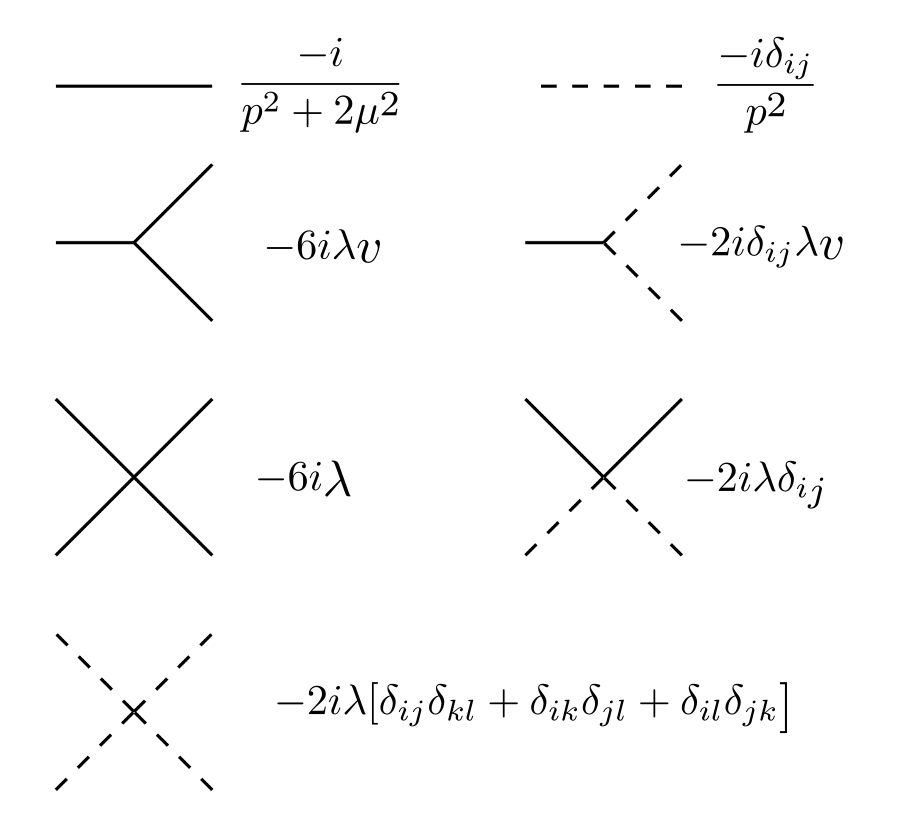
\includegraphics[height=6cm ,width=6.43cm]{QFT1/Li_sigma1.png}
\caption{Feynman rules for the linear sigma model}
\end{figure}

\noindent
Using these Feynman rules, we can compute tree-level amplitudes without difficulty. 
Diagrams with loops, however, will often diverge. For the amplitude with $N_e$ external legs, the superficial degree of divergence is
\[D = 4 - N_e\]
The linear sigma model has eight different superficially divergent amplitudes and several of these have $D > 0$ and therefore can contain more than one in nite constant.
\begin{figure}[!h]
\centering
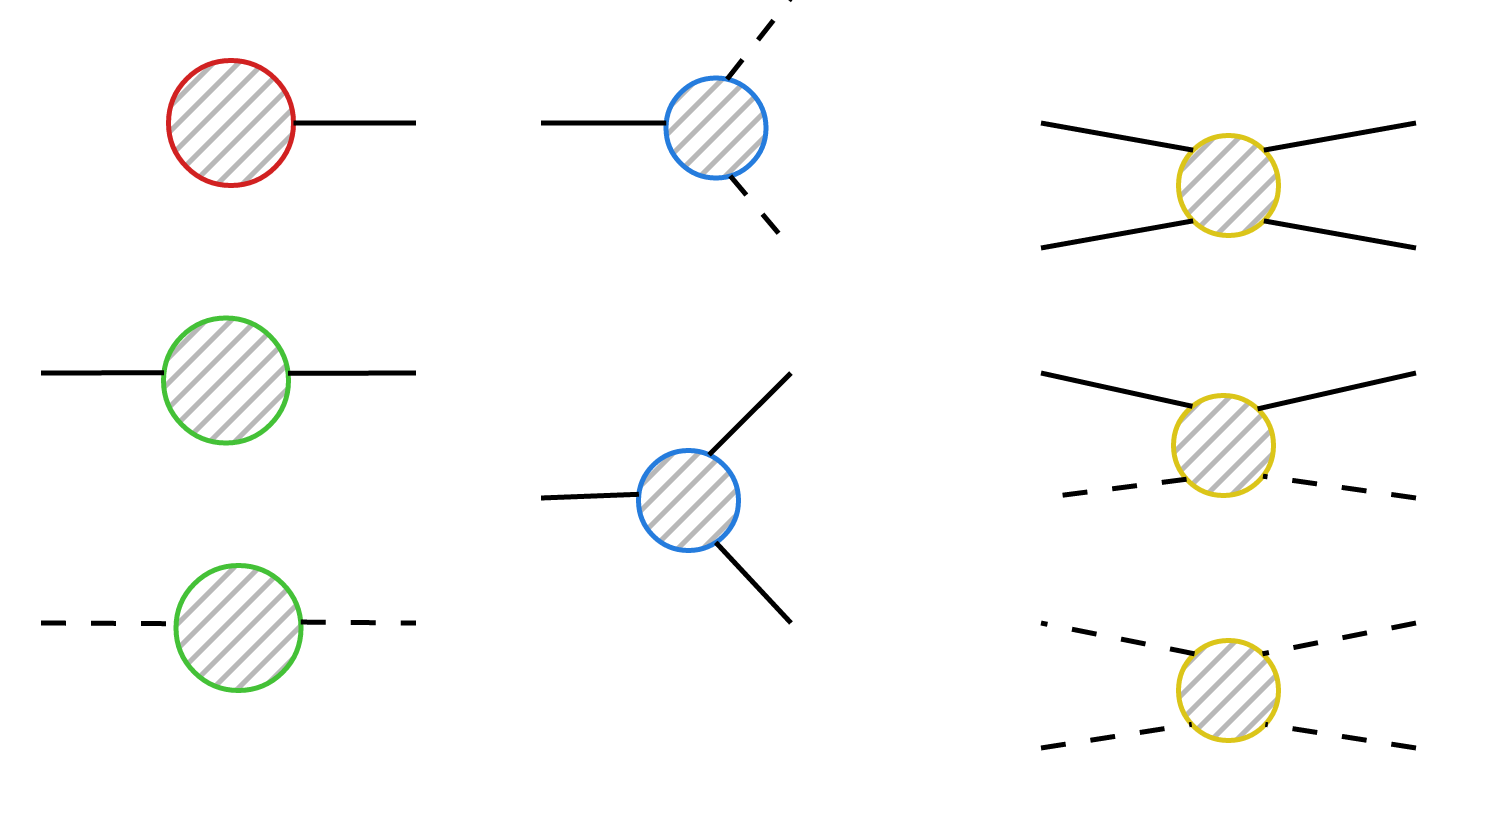
\includegraphics[height=4cm ,width=7.73cm]{QFT1/Li_sigma2.png}
\caption{Divergent amplitudes in the linear sigma model}
\end{figure}

\noindent
Yet we have only three counterterms:
\[\mathcal{L}_{ct} = -\frac{1}{2} \delta_Z \partial_{\mu} \phi^i \partial^{\mu}\phi^i - \frac{1}{2} \delta_{\mu} (\phi^i)^2 - \frac{\delta_{\lambda}}{4} [(\phi^i)^2]^2 \]
Written in terms of $\sigma$ and $\pi$ fields, we have
\begin{eqnarray}
\mathcal{L}_{ct} &=& -\frac{\delta_Z}{2}(\partial_{\mu}\pi^k)^2 - \frac{1}{2}(\delta_{\mu}+\delta_{\lambda}v^2)(\pi^k)^2 -\frac{\delta_Z}{2}(\partial_{\mu}\sigma)^2 - \frac{1}{2}(\delta_{\mu} + 3\delta_{\lambda}v^2)\sigma^2 \nonumber \\
&-& (\delta_{\mu}v + \delta_{\lambda}v^3)\sigma - \delta_{\lambda}v\sigma(\pi^k)^2 - \delta_{\lambda}v\sigma^3 - \frac{\delta_{\lambda}}{4}[(\pi^k)^2]^2 - \frac{\delta_{\lambda}}{2}\sigma^2 (\pi^k)^2 - \frac{\delta_{\lambda}}{4}\sigma^4 \nonumber
\end{eqnarray}
We can get the Feynman rules associated with these counterterms.
\begin{figure}[!h]
\centering
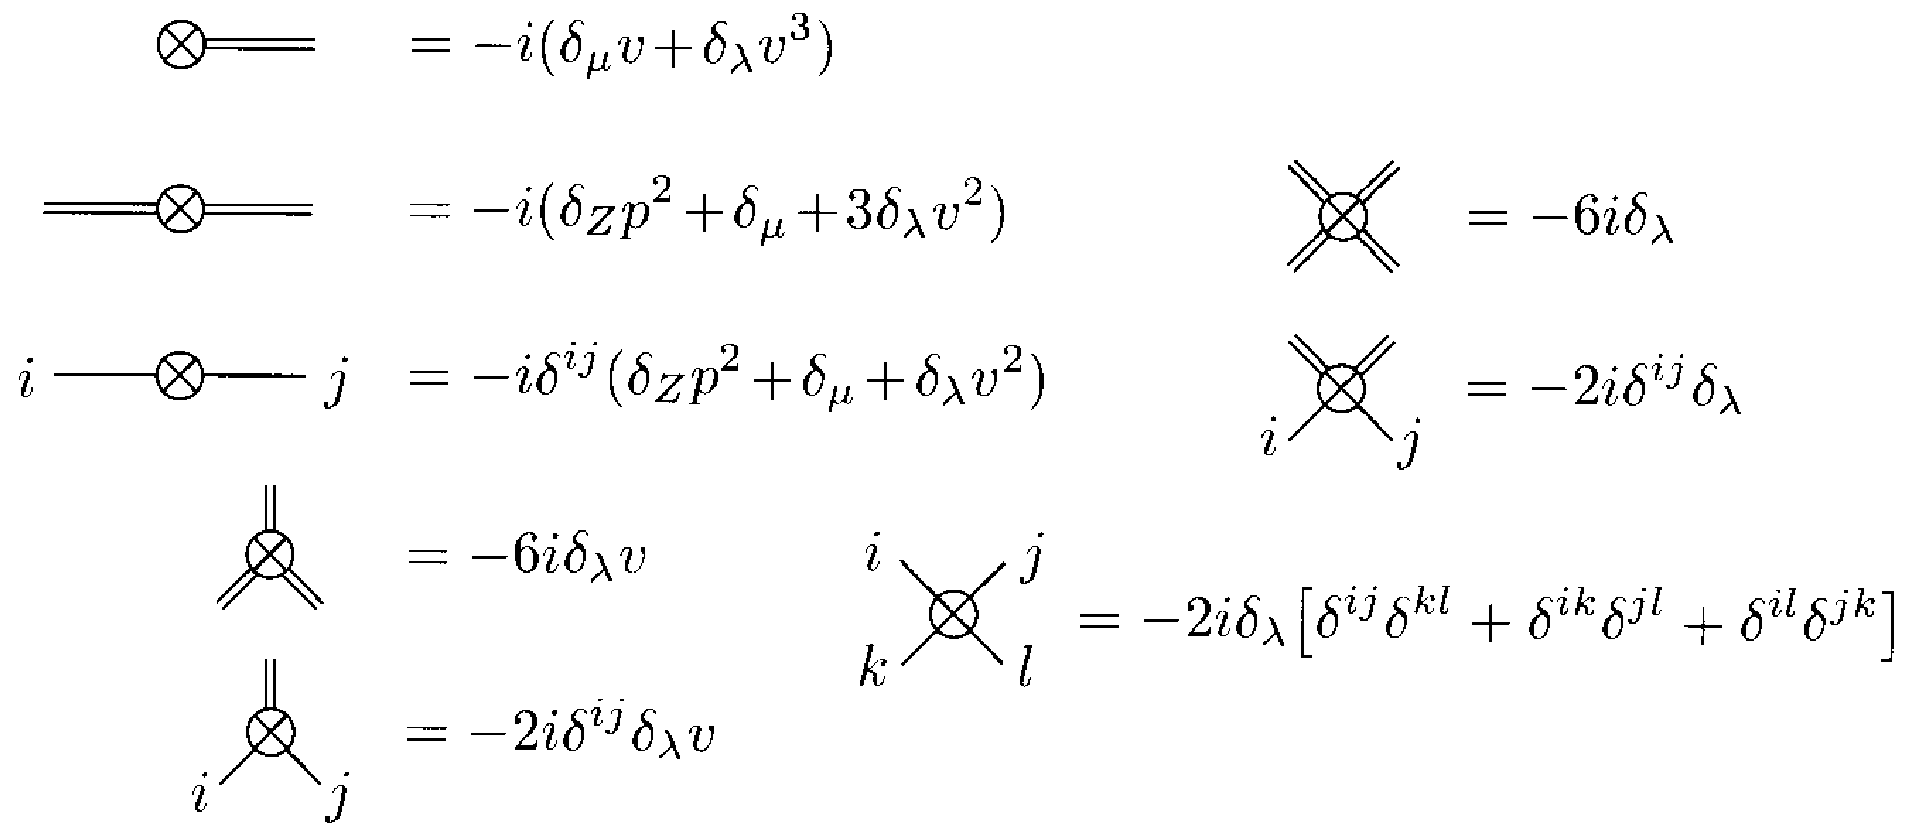
\includegraphics[height=5cm ,width=11.46cm]{QFT1/Li_sigma3.png}
\caption{Feynman rules for counterterm vertices in the linear sigma model}
\end{figure}

\begin{figure}[!h]
\centering
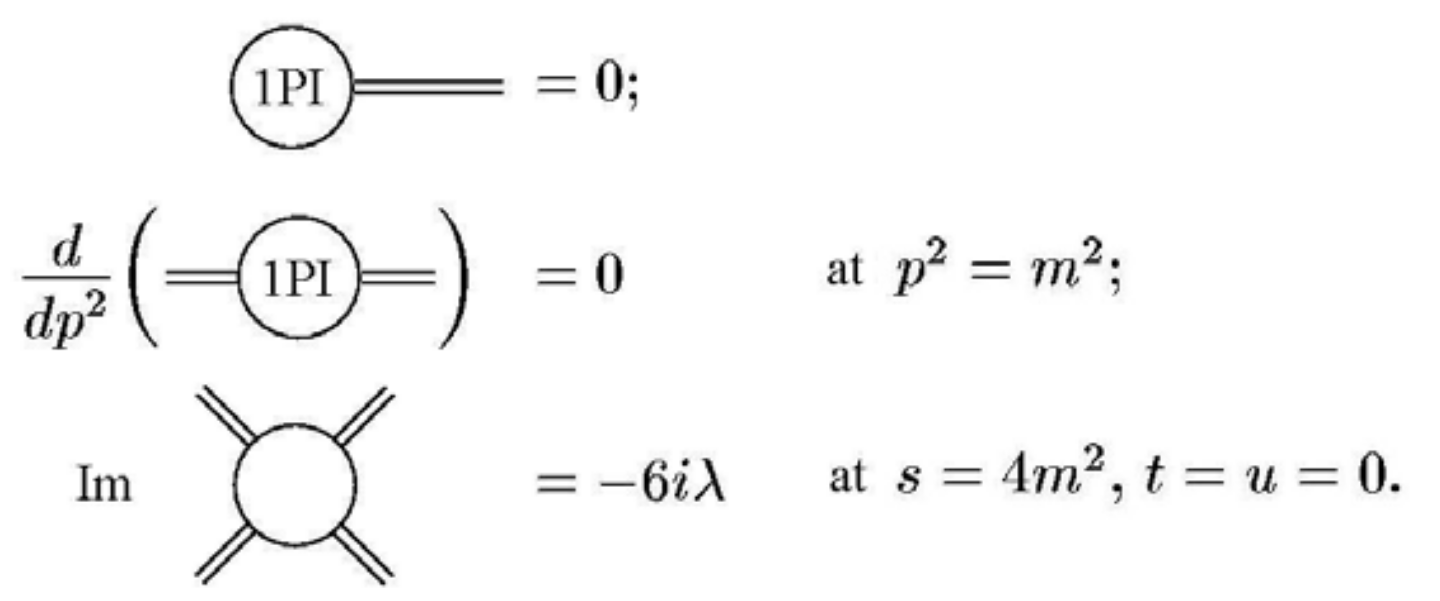
\includegraphics[height=3cm ,width=7.2cm]{QFT1/Li_sigma4.png}
\caption{Renormalization conditions ($m^2 = 2\mu^2$)}
\end{figure}

\noindent
Following the renormalization conditions above, the one-loop corrections for linear sigma model has been calculated in section 11.2 of \emph{An introduction to quantum field theory (M.E.Peskin \& D.V.Schroeder)}. There are two important results.
\begin{itemize}
\item All the divergence up to one loop will be cancelled by adjusting three counterterms. Apparently, the divergent part of the diagram is unaffected by the symmetry breaking.
\item The propagator of $\pi\pi$ has a pole at $p^2 = 0$ after one loop correction, i.e. $\pi$ particles remain massless after one loop correction.
\end{itemize}

\subsection{Effective action}
We begin again with the Lagrangian
\[\mathcal{L}_1 = -\frac{1}{2} \partial_{\mu} \phi^i \partial^{\mu}\phi^i + \frac{1}{2} \mu^2 (\phi^i)^2 - \frac{\lambda}{4} [(\phi^i)^2]^2\]
Expand about the classical field $\phi^i = \phi_{\mathrm{cl}}^i + \eta^i$, and we assume the vacuum is translational invariant. Then we have
\[\mathcal{L}_1 = -\frac{1}{2}(\partial_{\mu}\eta)^2 + \frac{1}{2}\mu^2(\eta^i)^2 - \frac{\lambda}{2}[(\phi_{\mathrm{cl}}^2)(\eta^i)^2+ 2(\phi_{\mathrm{cl}}^i\eta^i)^2] + \cdots\]
From the terms quadratic in $\eta$, we can read off
\[\frac{\delta^2 \mathcal{L}_1}{\delta\phi^i\delta\phi^j} = \partial^2\delta_{ij} + \mu^2\delta_{ij} - \lambda[(\phi_{\mathrm{cl}}^k)^2\delta_{ij} + 2\phi_{\mathrm{cl}}^i \phi_{\mathrm{cl}}^j]\]
We choose the vacuum state by demanding $\phi_{\mathrm{cl}}^i$ points in the $N$th direction
\[\phi_{\mathrm{cl}}^i = (0,\cdots,\phi_{\mathrm{cl}})\]
Then the operator is just equal to the Klein-Gordon operator $(\partial^2-m_i^2)$, where
\[m_i^2 = \begin{cases} \lambda\phi_{\mathrm{cl}}^2-\mu^2 \quad i=1,\cdots,N-1 \\ 3\lambda\phi_{\mathrm{cl}}^2-\mu^2 \quad i=N \end{cases}\]
The calculation of functional determinant will be covered in the next chapter, and you can check the section 11.4 of \emph{An introduction to quantum field theory (M.E.Peskin \& D.V.Schroeder)} for the details. Here, we list the final result
\[\log\det [-\partial^2 + m^2] = -i\frac{\Gamma(-\frac{d}{2})}{(4\pi)^{d/2}}(m^2)^{\frac{d}{2}}VT\]
So, up to one loop corrections.
\[V_{\mathrm{eff}} = -\frac{1}{2} \mu^2 \phi_{\mathrm{cl}}^2 + \frac{\lambda}{4} \phi_{\mathrm{cl}}^4 - \frac{1}{2}\frac{\Gamma(-\frac{d}{2})}{(4\pi)^{d/2}}[(N-1)(\lambda\phi_{\mathrm{cl}}^2-\mu^2)^{\frac{d}{2}} + (3\lambda\phi_{\mathrm{cl}}^2-\mu^2)^{\frac{d}{2}}] + \frac{1}{2}\delta_{\mu}\phi_{\mathrm{cl}}^2 + \frac{1}{4}\delta_{\lambda}\phi_{\mathrm{cl}}^4\]
And if we want $V_{\mathrm{eff}}$ is finite for terms involving $\phi_{\mathrm{cl}}$, we can get
\[\delta_{\lambda} = \frac{2\lambda^2(N+8)}{(4\pi)^2} \times \frac{1}{4-d} + \mbox{ finite terms }\]
\[\delta_{\mu} = -\frac{2\lambda\mu^2(N+2)}{(4\pi)^2} \times \frac{1}{4-d} + \mbox{ finite terms }\]
It is the same result as that in previous section.